\documentclass{art}
\usepackage{pict2e}
\usepackage{shorttoc}
\usepackage{xspace}
\usepackage{color}

%Stuff I'm using you may want to redefine in the style
% \emph, \begin{verbatim},
% section names
% sec:introduction
% sec:quickstart
% sec:beforeyoubegin
% sec:installing
% sec:usingart
% sec:background
% sec:developing
% sec:gnustep

%\title{ART \\
%\small\emph{The Advanced Rendering Toolkit Installation and Operation Manual} \\
%Version 1.6}
%\date{$ $Date: 2006/03/31 13:03:02 $ $} % date entry will come from CVS

%\author{%
%  \begin{tabular}{ll}
%    Alexander Wilkie     & Christiane Ulbricht  \\
%    Caroline Larboulette & Georg Zotti
%  \end{tabular}
%}

% keep this up-to-date!
\newcommand{\rem}[1]{\texttt{[#1]}}
\newcommand{\term}[1]{\textit{#1}} %was: without number, simple  {\emph}
%\newcommand{\textcircle}[1]{\textbf{(#1)}}
\newcommand{\textcircle}[1]{\textcircled{\small{#1}}}
%\newcommand{\textcircle}[1]{$\hspace*{1pt}$ $\put(2.1,3.075){\circle{9}} #1 $  $\hspace*{1pt}$}
\newcommand{\vs}{vs.\@\xspace}
\newcommand{\ie}{i.e.\@\xspace}
\newcommand{\eg}{e.g.\@\xspace}
\newcommand{\ea}{et~al.\@\xspace}
\newcommand{\aso}{aso.\@\xspace}
\newcommand{\etc}{etc.\@\xspace}
\newcommand{\resp}{resp.\@\xspace}
\newcommand{\eae}{\ea\xspace}
\newcommand{\cf}{cf.\@\xspace}
\newcommand{\mycite}{~\cite}
\newcommand{\luv}{ $L^*u^*v^*$ }
\newcommand{\rgb}{RGB }
\newcommand{\xyz}{XYZ }
\newcommand{\ciexyz}{CIE XYZ }
\newcommand{\cielch}{CIE LCH }
\newcommand{\cielab}{CIE $L^*a^*b^*$ }
\newcommand{\UnivProf}{Univ.~Prof.\@\xspace}
\newcommand{\UnivAss}{Univ.~Ass.\@\xspace}
\newcommand{\Dr}{Dr.\@\xspace}
\newcommand{\DI}{Dipl.--Ing.\@\xspace}
\newcommand{\Nr}{Nr.\@\xspace}
\newcommand{\zB}{z.B.\@\xspace}

\newcommand{\Part}[1]{\clearemptydoublepage\part{#1}}
\bibliographystyle{alpha}
\begin{document}


\thispagestyle{empty}

{\Huge The ART Handbook}\\
\vspace{1.5cm}

\emph{The Advanced Rendering Toolkit}\\
\emph{Installation, Usage, and Technical Information}\\

\vspace{1.5cm}
%Version 1.8 -- $ $Date: 2006/03/31 13:03:02 $ $ % date comes from CVS
\input{timestamp}
\vfill

\vspace{10cm}
{\centering
\begin{tabular}{>{\scshape }l>{\scshape }l}
Alexander Wilkie & Andrea Weidlich \\Alban Fichet & Michal Mojzik \\
 \\
Typesetting: Georg Zotti        \\
\end{tabular}
\vfill
}

%\maketitle
%\shorttableofcontents{Overview}{0}
\thispagestyle{empty}

\clearemptydoublepage
\section*{Introduction}
\label{sec:introduction}

In this document, we describe installation and operation of
the 2.x series of the Advanced Rendering Toolkit (ART). ART is a
Predictive Rendering research system developed mainly by the graphics group of Charles University, Prague, Czech Republic. ART is actually quite old: its development roots can be traced back to the year 1996, and the Institute of Computer Graphics in Vienna, Austria, where it was originally conceived by Robert F. Tobler\footnote{An outline of the development history of ART can be found in section~\ref{sect:arthistory}.}.

The 1.x series of ART was never released to the public, but served as the base from which current ART 2.x was developed. ART 2.x shares many core features with ART 1.x, but is also a hopefully much more consistent and maintainable codebase than version 1.x. However, as part of the inevitable re-factoring that led to ART 2.x, a number of interesting features of ART 1.x have not been ported yet: hopefully, as time progresses, most of these will be added back.

The document is composed of three main parts: 

\begin{description}
\item[Part I] a \emph{getting started} guide, which aims at describing how to install
  and run ART,
\item[Part II] which contains general information about some internal concepts and the design
philosophy of ART, and
\item[Part III] which specifically contains information about the spectral rendering and polarisation capabilities of ART.
\end{description}


Please report any typos, inaccuracies or problems to the project mail address:\\
\mailto{art@cgg.mff.cuni.cz}


A current version of this document can always be found in the Documentation
directory of the ART source tree \filename{(\envvar{ART\_DIR}/Documentation)} under the name
\filename{ARTforNewbies.tex}. Enter this directory and type \command{make pdf} to create a version of this PDF which matches the release you have on your computer.
\thispagestyle{empty}

\clearemptydoublepage
\tableofcontents

\setcounter{page}{-1}
\Part{Getting Started With ART}
\chapter{Getting Started}
\label{sec:beforeyoubegin}
\section{System Requirements}
ART can basically be built and run everywhere where one can get a
modern Objective C compiler to build and run. The only real external dependencies are a
\command{gcc} version $4.2$ or better\footnote{Currently, \command{gcc} 4.6 or better is desirable, since it fixes an annoying bug that generated lots of incorrect warnings about protocol support. But apart from the spurious warnings (which can be distracting if you are trying to debug something, and want to find real errors and warnings), \command{gcc} $4.2$ is also capable of building a working copy of ART.} or \command{llvm} with Objective-C support,
\command{git}, \command{cmake} in version 2.8 or greater\footnote{On OS X, you actually need \command{cmake}~2.8.6 or greater - lower versions have broken Xcode support.}, Sam Leffler's TIFF library (\ie \textit{the} common \command{libtiff}), and version 2 or greater of the \command{litteCMS} library (\url{http://www.littlecms.com/}). On Linux, you will also need GNUStep (\url{http://www.gnustep.org/}) installed. 

Optional but highly recommended is the OpenEXR library (\url{http://www.openexr.com/}). If the latter is not present, ART of course cannot read or write EXR images, but is otherwise functional. Note that ART has its own internal HDR image formats, so EXR capabilities are not a critical requirement for getting renderings done. However, if you want to share results with anyone outside the project, EXR is the de facto standard for HDR images.

\section{Getting the Source}
At the moment the standard way of obtaining the ART sources is via the
git repository of the project. This method is greatly favoured over all
others (in particular the distribution of source tarballs) since it
makes both the incorporation of changes done by project collaborators
much easier, and also provides an easy way for users to upgrade their
installation to new versions.

\subsection{Git Repository Clone}

There are two ways to obtain the source: either via anonymous \command{git} access via

\begin{verbatim}
git clone git://cgg.mff.cuni.cz/ART.git
\end{verbatim}

which provides you with a local repository that you can work with: so you can even make local commits, and use the local git repo for your own experiments with the code. However, you cannot write anything back to our server.

For our collaborators (and only those - see the FAQ on the project website), there is also an option to access the git repo via \command{ssh}. If you are one of those to whom we give such access, we will need your public ssh key identity to establish your credentials on the server. Once these are installed, you can interact with the server without any password entry. Once you have your account, you can check out the sources for ART via the following command:
\begin{verbatim}
git clone ssh://git@cgg.mff.cuni.cz/ART
\end{verbatim}

Either way, the first step of working with ART is now complete - you now have a local repository of
the project.

\subsection{Collaborators: working on your own Git Branch}
\label{sec:forking}
If you are going to do any sort of development work on ART, you are required to work on your own branch at all times. Making any direct changes to the master branch, and in particular, pushing such changes back to the project server, is strictly forbidden! So the very first thing you should do after cloning the repository is to change to your own branch via the command
\begin{verbatim}
git checkout -b <your branch name>
\end{verbatim}
This command has the issued from within the project directory you just cloned. Obviously, you have to replace \command{<your branch name>} with a suitable branch name of your own: a combination of username and and an acronym of the feature you are working on is a reasonable thing to use here.

Merging any changes you make into the current project master requires explicit authorisation from the project maintainer, and is only permissible if the merged version passes the regression test suite.

%%% Local Variables:
%%% mode: latex
%%% TeX-master: "ARTforNewbies"
%%% End:

\chapter{Building ART}
\label{sec:installing}

The actions you have to take to obtain a running installation of ART can be
split into three categories: things which have to be done only once (regardless
how many checkouts of ART you perform), stuff you have to repeat only if you
obtain a completely new copy of ART (\emph{not} after each git pull in an existing repository clone), and
things you have to do each time you make changes to the libraries (the recompile
which is necessary to update the executables).

For users who just use ART to generate images, all these steps only have to be
performed once.

\section{Stuff You Only Have to Do Once}


\subsection{Making Sure the Executable Path is Correct}

For ART to work properly, the place where the executables will be installed has to be on the search path. If you work locally with ART (\ie within your user account), this amounts to having \filename{\textasciitilde/bin} in your path. Many people already have that anyway, but if you have not, add something like

\begin{verbatim}
path=(~/bin/ $path)
\end{verbatim}

to your shell startup file (the exact syntax will depend on the shell you use). If you install ART in any of the canonical system-wide locations, you do not have to do anything in pretty much all modern Unices.

\subsection{Specifying the Results Viewer}

There is one more environment variable you might want to consider setting. It controls which viewing program is used to display the results of a rendering job or tone mapping operation, \ie open the resulting picture. ART has sensible defaults built in for the various platforms it can be compiled on, but you might still want to override those to use the viewer program of your choice, especially on Linux. On OS X, ART defaults to using the \command{open} command, which already uses the GUI preferences for each filetype; changing this does not make much sense. You still can, of course -- even on OS X, the environment variable is read. But on Linux (and other Unices), directly specifying an alternate viewer executable can be desirable. You can do that by putting

\begin{verbatim}
export ART_VIEWER=<exectuable of your choice>
\end{verbatim}

in your shell startup file.

\subsection{Specifying ART environment variables}
In case you're choosing to build ART in a different path than \verb?~? or \verb?\usr?, you need to specify some environment variables to enable ART to run: \verb?ART_RESOURCE_PATH? and \verb?ART_LIBRARY_PATH?.

For example, if you've chose to run CMake with \verb?-DCMAKE_INSTALL_PATH=~/art?, your should set the following environment variable like so:

\begin{verbatim}
export ART_RESOURCE_PATH=~/art/lib/ART_Resources                                                                                                                              
export ART_LIBRARY_PATH=~/art/lib
\end{verbatim}
%export LD_LIBRARY_PATH=~/art/lib:$LD_LIBRARY_PATH
%export PATH=~/art/bin:$PATH 

\subsection{Issues specific to Linux}

\subsubsection{Setting the Dynamic Library Path}

If you install ART in a system-wide fashion, you are set -- nothing else needs to be done. If you are using Linux, and the finished ART is going to live in your home directory, though, you have to set one environment variable so that the dynamic linker finds the shared library you build:

\begin{verbatim}
export LD_LIBRARY_PATH=~/lib:$LD_LIBRARY_PATH
\end{verbatim}

\subsubsection{If Needed: Override the Command Line Locale Setting}

Linux comes in many flavours, and some of them have less than sensible ways of handling localisation. One potential issue in this regard is that for European or other non-US locations, alternate floating point number formats are sometimes used even for command line applications. Whether this affects you depends on your locale settings and your particular Linux: what you should check for is whether floating point numbers are printed using dots ("{\tt 1.0}" - US/EN) or commas ("{\tt 1,0}" - DE, CZ, and others) as decimal delimiters. ART expects the decimal delimiter to be a dot, and does not work correctly if commas are used. So if you see commas in floating point numbers, please override the locale settings for the command line environment you are in:

\begin{verbatim}
export LC_ALL=en_US.UTF-8
export LANG=en_US.UTF-8
export LANGUAGE=en_US.UTF-8
\end{verbatim}

\section{Stuff You Only Have to Do Once for Each New Source Check-Out}

\subsection{Run CMake}

The only decisions you have to make at this point is whether you want to install the finished ART binaries globally for all users (which usually requires you to have \command{sudo} rights), or if you want to keep ART within your home directory. The latter option is the sensible choice for active developers. To make the choice, go to the source directory, and type either

\begin{verbatim}
cmake .
\end{verbatim}

to configure ART for eventual system-wide installation, or

\begin{verbatim}
cmake . -DCMAKE_INSTALL_PREFIX=~
\end{verbatim}

to build and install it in your home directory. CMake does all the rest for you.

\subsection{Issues specific to OS X}

On OS X, you have to create an Xcode project from the sources; this builds a framework that is again either installed globally (see above -- requiring you to have \command{sudo} rights), or locally within your account. Create the project file for a local installation with

\begin{verbatim}
cmake . -G Xcode -DCMAKE_INSTALL_PREFIX=~
\end{verbatim}

Global installations of ART under OS X of course omit the \command{-DCMAKE\_INSTALL\_PREFIX}. Open the resulting Xcode project, and take it from there.

\section{The Actual (Re-)Building of ART}
\label{sec:Installing:Building}
\label{sec:Installing:Building:Rebuilding}
Under Linux, compilation of the entire ART sources, either from scratch, or after changes have been made to the sources, is straightforward:
\begin{verbatim}
cd <ART source directory>
make
make install
\end{verbatim}
On machines with two or more processors the compilation can be speeded up
significantly by specifying the option \option{-j<n>} to use $n$ processors in
parallel, e.g.
\begin{verbatim}
make -j2 
\end{verbatim}
on a dual processor workstation. In any case the compilation should be expected to take a bit of time -- but on fast multiple processor workstations a complete build takes a few minutes at the most.

On OS X, you use Xcode to build the Advanced Rendering Toolkit framework, and the associated binaries. Make sure you use the target "install", and that you have added the target directory to the executable path of your shell.


%%% Local Variables: 
%%% mode: latex
%%% TeX-master: "ARTforNewbies"
%%% End: 

\chapter{Using ART}
\label{sec:usingart}

ART is a toolkit which provides several command-line
applications. These all perform smaller, individual tasks that are relevant to
photorealistic image synthesis, following a UNIX-like philosophy: there is no single large application, but rather several smaller, modular ones.

Since its inception, ART has been a command-line only toolkit since
\begin{enumerate}
\item we wanted to concentrate on getting the implementation of the
  photorealistic rendering processes right without having GUI issues standing
  in the way and
\item we neither wanted to be tied to one particular GUI that we would have to
  develop for, nor be burdened with some kind of portable cross-GUI solution.
  These only became viable long after ART was started, and we might integrate
  one yet sometime.
\end{enumerate}

Once the toolkit has been built and installed with \command{make install} (or the \command{install} target in Xcode), ART
is ready for use. It installs its executables as specified to \command{cmake}. Usually, when doing development work local to your account, they are placed in \command{\textasciitilde/bin}. Currently the three main applications are: \command{artist} (the actual command-line renderer), \command{tonemap} (the
tonemapping tool) and \command{bugblatter} (the difference image generator), but there are others as well.


Calling each of them without any arguments displays information about the version of the particular executable which is being called. If you call any of them with the option \command{-h}, all the valid soptions for this particular application are displayed.

\section{Usage Background}
We first outline some general points about the design philosophy of ART applications, and then briefly discuss the fairly simple actual usage of the tools.

\subsection{Action Sequences}
\label{sec:using:ActionSequence}
Rendering jobs in ART were intended to go beyond the traditional rendering toolkit workflow of
\begin{quote}\itshape
the user provides a scene which just contains some geometry, and does
  everything else by first fiddling around with the hardwired command-line
  parameters of the actual renderer, and later perhaps calling the tone mapper
  on some HDR result image.
\end{quote}


Anything which is done by an ART command line application is determined by a so-called \emph{action sequence} that is executed. With the exception of \command{impresario} (which makes no use of action sequences), the only real difference between the various ART command line applications lies in where the action sequence they execute comes from, and at which point of the rendering pipeline it starts.

Action sequences are linearly progressing, non-branching lists of \class{ArnAction}-derived object instances. They
are stored in an \class{ArnActionSequence} object, and are executed one after another. Each action can
take arbitrarily many \emph{data objects} off the provided single \emph{data stack}. This stack is initialised according to the task at hand: for rendering purposes, the camera, the -- at that point, still empty! -- result image, and the scene geometry are initially placed there. The tone mapper initialises it by putting the raw images that are to be processed there, while the image comparison tool initially pushes the two images that are to be compared. Each action in the sequence then works by taking the input it needs from this stack, and places any resulting objects back there. If an action does not find the data object(s) it needs on the data stack, it terminates the program with an error message.

The utility of this concept is easily seen when considering what has to be done for a typical rendering job to arrive at the desired end result of a displayable RGB image: 
\begin{itemize}
\item loading of the scene into memory
\item insertion of raycasting acceleration structures, e.g.\ bounding
  boxes
\item identification and measurement of the lightsources
\item the actual rendering, e.g.\ path tracing -- this yields an intermediate \command{artraw} HDR image, a lossless format internal to ART
\item conversion of the (possibly spectral) \command{artraw} image to the equally lossless
  colour space HDR format \command{artcsp}
\item tone mapping
\item gamut mapping
\item conversion from the \command{artcsp} format
  to a common end-user image format, such as TIFF.
\end{itemize}

The various actions in this sequence perform different data stack manipulations;
for instance, the second one takes the plain scene graph off the data stack,
inserts the bounding boxes and puts it back. The lightsource analysis action
first pops the scene graph off the data stack, analyses it, and then puts it back
again, along with a collection of lightsource descriptors in a separate
container object. The path tracing action expects a camera, a scene graph and a
collection of lightsource descriptors on the data stack, and puts an
\filename{artraw} image back. And so on.

Apart from compartmentalising the parameters for each of the subtasks necessary
for image synthesis this approach also allows easy modification of the process:
a nice example would be to exchange the action which inserts bounding boxes
against one which inserts a kD-tree. Since the raycaster used by the path tracer
is oblivious to what---and indeed if any---ray acceleration data structures are
present (with the obvious exception from the user's viewpoint that execution
times skyrocket if there are none) this provides a highly intuitive way of
comparing the performance of different algorithms.

Normally, an action sequence is assembled on the fly based on the command line options specified by the user (most applications, such as \command{tonemap} or \command{bugblatter}, follow this pattern), or loaded together with the scene file (as with the actual renderer, \command{artist}). In addition to this, a lot of ART command line applications have the option \command{-acs <filename>} to load an entire, ready-made action sequence from disk; this overrides any in-built action sequences, or those found in a scene file. This capability is convenient if systematic manipulation of large numbers of files is desired, and saves the bother of always having to specify lots of command line parameters. But there are also some mono-purpose tools such as \command{bugblatter} which cannot load a complete action sequence from disk. Internally, however, even the mono-purpose tools use a small action sequence, and the \command{-acs <filename>} functionality could easily be activated for them.

\subsection{The Structure of an ART Scene}
ART uses a proprietary scene description language not out of the desire to
invent yet another file format, but rather for various hard technical reasons,
one of them being for instance the fact that no existing format provided the
possibility to properly incorporate (bi-)spectral reflectance and emission data. 

Another key reason---\emph{the} reason as far as this part of the explanation is
concerned---was that a file format which is capable of encoding the entire
rendering pipeline after the modeling step was deemed to be a desirable
property. This is achieved by saving the associated action sequences as integral
part of each ART scene---and thereby storing instructions for all manipulation
steps apart from the actual rendering alongside the geometry.

The top-level object in any ART scene is of the type \class{ArnScene},
an Objective-C class which maintains the geometry, the camera, an
environment map / skydome description (if present) and the action sequence. This is also
the kind of class many actions expect on the data stack---just putting
plain geometry there would not work.

The user-editable format of such native ART scenes is the
\filename{.arm} format (which cannot be directly parsed by the
renderer), whereas the internal, parseable versions of these scenes
are \filename{.art} or \filename{.arb} files. Details on the
relationship between these formats can be found in background
section~\ref{sec:ARTscenefileformat}.



\section{Using the Renderer}
%The \command{artist} executable has always had the idiosyncrasy that it only
%works properly when called from its application directory. Fixing this would not
%require a major effort (it would mainly require that \command{artist} gets some
%notion of library search paths---not exactly rocket science), and will probably
%occur sometime in the nearer future.

The minimal action to render the scene described by the file \filename{foo.arm} is to change into the directory where the scene \filename{foo.arm} lives, and invoke \command{artist}:

\begin{verbatim}
cd <working dir>
artist foo.arm
\end{verbatim}

As long as no GUI scene editor for the actual internal \filename{.art} scene file format exists, changing anything in the scene has to be done by editing the associated \filename{.arm} file. 

\subsection{Multiprocessor Operation}
On being started up, the ART libraries detect the number of available processor cores, and use all of them where this is applicable and implemented. This behaviour can be overridden via the option \option{-j~<n>} to use $n$ processor cores ($n$ can be either larger or smaller than the number of physical cores - use this at your discretion).

Note that ART at the moment only uses threading for some of the cases
where this is possible; as development progresses this ratio will
increase. The major tasks -- such as the actual path, photon or ray
tracing -- are threaded, but there is still room for improvement,
especially during the scene setup phase (\eg lightsource
identification or mesh preparation calculations).

\subsection{Obtaining Intermediate Rendering Results}
For reasons of efficiency, \command{artist} does not write any intermediate results to disk while it is running. The rendering thread(s) store all computed information locally in each thread: only once all of them have terminated, the complete result image is assembled by the main thread, and saved to disk. 

For long-running rendering jobs, this behaviour can be undesirable, as one might want to quickly see whether the rendering is doing what one expects. To solve this problem, it is possible to obtain intermediate results at any time during rendering with the \command{impresario} command. This small tool uses UNIX signals to wake up the dormant main thread of a running \command{artist} instance, and forces it to write (and if selected, also display) the current state of the result image. \command{impresario} can also be run in a way that it sends repeated wake-up calls to \command{artist} at pre-defined time intervals.

\subsection{Changing the Result Image Size}
\label{sec:using:imageSize}
Sometimes it is desirable to alter the size of the output image---or
to render just a subimage---without altering the scene file itself.

The option \option{-res WxH} will create an output image $W$ pixels
wide and $H$ pixels high.  The option \option{-res /r} reduces the
size of the output image by the factor $1/r$, and the options
\option{-x x0:x1} and \option{-y y0:y1}, which---used individually or
together---restrict image synthesis to the subimage defined by
$(x_0|y_0)$ and $(x_1|y_1)$.  

Examples would be
\begin{verbatim}
artist foo.arm -x 0:20 -y 30:40
\end{verbatim}
which only renders the subimage bounded by the points ($0|30$) and ($20|40$) and
\begin{verbatim}
artist foo.arm -res /2
\end{verbatim}
which renders the image at half the resolution specified in the scene
file. Enlargement is also possible by specifying fractions, as in
\begin{verbatim}
artist foo.arm -res /0.5 
\end{verbatim}
which yields a result image of twice the original size. This slightly
counterintuitive notation is necessary since most (probably all) shells escape
(i.e.\ for our purposes hide) the \option{*} character which would be the far more
obvious choice here.

Also note that the resolution change and subimage options can be
combined, and that the \option{-x} and \option{-y} subimage options
already operate on the altered size of the image in that case (i.e.\ 
you have to specify the subimage coordinates in terms of the new image
size).  Note further that one of either $x_0, x_1$ or $y_0, y_1$ can
also be omitted, meaning ``from edge to given value''. So, the
following command can be used to produce a section in the top right
corner of a reduced image:
\begin{verbatim}
artist foo.arm -res /4 -x 20: -y :25
\end{verbatim}

\subsection{Passing \command{\#define}s to \filename{.arm} Files}

As explained in depth in section~\ref{sec:ARTscenefileformat}, all human-editable \filename{.arm} input files are automatically translated into the internal \filename{.art} format before use. This process is usually very quick, and involves compilation and execution of the \filename{.arm} file. As the human editable scene files of ART are basically Objective-C programs, it is possible to transparently pass \command{\#define}s to them from the command line, in a manner similar to \command{gcc} or \command{llvm} command-line behaviour. The purpose of this facility is to be able to control certain frequently modified scene file properties, such as the number of samples that are to be taken for each pixel, via the command line, without having to edit the actual scene file.

For example, if the scene file \filename{foo.arm} uses a conditionally defined macro \command{SAMPLE} to define a default number of samples cast for each pixel, like this:

\begin{verbatim}
#ifndef SAMPLES
#define SAMPLES 32
#endif
\end{verbatim}

it can then later be used during the definition of the scene action sequence, in the spot where sample count is specified (see the scene files in the ART Gallery for examples):

\begin{verbatim}
[ STOCHASTIC_PIXEL_SAMPLER
	...
    samplesPerPixel:  SAMPLES
    ],
\end{verbatim}

This value can then be conveniently over-ridden from the command line: all \command{-D} switches force re-translation of the \filename{.arm} file, so the scene is automatically re-translated with \command{SAMPLE} set to 256:

\begin{verbatim}
artist foo.arm -DSAMPLES=256
\end{verbatim}

Note that this facility is not limited with regard to the number of \command{\#define}s that are passed to the \filename{.arm} file before translation: so you can be creative in making your scenes capable of command line manipulation via as many such switches as you want. Note also, though, that there is currently only an informal standard on what conditionally defined macros one can expect in an \filename{.arm} file: all examples in the ART gallery use \command{SAMPLE} to define the number of samples, and a number of them have an option \command{DIFFUSE\_ILLUMINATION} that can be activated instead of the standard scene illumination. But beyond that, there are no conventions at the moment.

\subsection{Tagging Output by Data Type}
Note should also be taken of the \option{-t} option, which tags the output of a
rendering pass with the name of the data type that is used for the pixels of the image. For example,
rendering the scene \filename{foo.arm} with the \option{RGB} renderer and
the \option{-t} flag set would generate a result file of the form
\filename{foo.RGB.tiff}, while a polarising \option{Spectrum8} rendering would yield
\filename{foo.Spectrum8.polarising.tiff}.

This is useful for those users who wish to compare e.g. colourspace and spectral renderings of the same scene, or the effect of different spectral output resolutions: one can easily keep the results of these computations in separate files this way. 


\subsection{Tagging Output with an Arbitrary Tag}
The option \option{-tt <extraTag>} allows you to give yet one more tag
to the filename.  \option{.<extraTag>} is added just before the
filename extension. Useful tags typically may be things you are currently
testing, like number of samples, recursion depth, filter names, \ldots

Note that \option{-tt} can of course be combined with \option{-t}, so that

\begin{verbatim}
artist foo.arm -t -tt TestCase1
\end{verbatim}

would yield an output file named \filename{foo.Spectrum8.TestCase1.tiff}. In normal operation, you probably do not need this sort of thing, but it can be very handy if you \eg do systematic experiments, and wish to tag the images properly in order to be able to tell them apart later.

\subsection{Generating High DPI Result Images}
The option \option{-ret} doubles the DPI count of result images, to yield images that "natively" display on modern high-DPI displays ("Retina displays"). Selecting this option also automatically doubles image resolution, and thereby likely quadruples rendering time. However, on modern displays, a much sharper image results. Use this feature with care when appropriate.

\section{Using the Tonemapper}

The \command{tonemap} executable is a tool designed to cover the last third of the rendering pipeline -- all that which comes after image synthesis. Currently, it is capable of reading and processing \filename{ARTRAW}, \filename{ARTCSP} and (if ART was built with support for the format) \filename{EXR} images. Usage is straightforward: the name of the image you want to process, followed by the desired tone reproduction operator, together with parameters:

\begin{verbatim}
tonemap foo.artraw -iac -a 1 
\end{verbatim}

which yields an \filename{RGB TIFF} version of the \filename{ARTRAW} image in
question, using the Interactive Calibration tone reproduction operator, with the algorithm parameter $a$ set to 1. Use \command{tonemap -h} to see a list of all available tone mapping operators and output options. Note that different RGB spaces are available for the final output image (Wide Gamut RGB might be suitable for very colourful images in some cases), as well as the option to generate 16 bpc \filename{TIFF} images.

\section{Bugblatter: Creating Difference Images}
\label{sec:using:bugblatter}

This application generates difference images between two \filename{ARTCSP} images, which obviously have to be of the same size:

\begin{verbatim}
bugblatter foo.artcsp bar.artcsp -o snarfle
\end{verbatim}

This generates a difference image of the two images \filename{foo} and \filename{bar}, and names the resulting image \filename{snarfle}. Use \command{bugblatter -h} to see a list of available options.

The \filename{ARTCSP} files needed for this comparison can easily be obtained by using the \command{-rcsp} option of \command{tonemap}. This option retains the last intermediate \filename{ARTCSP} file before conversion to some common image format (\filename{TIFF}, \filename{EXR}). The output options are very similar to those for \command{tonemap} (16 bit output, RGB colourspace selection, \etc).

\section{Polarisation Visualisation}
As ART is capable of rendering with polarised light, and of storing the results in spectral image files that actually contain polarised light for each pixel, a tool to visualise these results named \command{polvis} is included with the toolkit. Much like \command{tonemap}, it is a command-line application that offers the sort of output options that are common to all ART image processing tools. Unlike most other tools, \command{polvis} is specific with regard to its input insofar as it will refuse to work on non-polarised \filename{ARTRAW} files.

The visualisation options are pretty much exactly those outlined in the 2010 SCCG paper "A Standardised Polarisation Visualisation for Images": degree of polarisation (option \command{-dop}), prevalence of linear versus circular polarisation (\command{-lvc}), orientation of linear polarisation (\command{-lin}), as well as the chirality of any circular polarisation that may be present (\command{-cir}). In addition to these "canonical" four plots, there is also a fifth option that splits the image into its four Stokes Components, and outputs these separately as four false-colour images (\command{-stc}).

For all of the four "canonical" plots, three display options exist: stand-alone (the default behaviour, with a black background), and two that are overlaid over a black and white version of the ARTRAW image in question (see the 2010 paper for details). The black and white image is actually not a normal black-and-white conversion of the image in question, but a monochrome spectral image extracted at the visualisation wavelength. So, to give just one example, a \command{polvis} invocation like this

\begin{verbatim}
polvis foo.artraw -dop -so -wl 400
\end{verbatim}

would yield a degree of polarisation plot for wavelength 400nm, that is overlaid over a tone mapped black and white version of the image at that wavelength. The resulting visualisation would have the filename

\begin{verbatim}
foo.dop.400nm.scaledOverlay.tiff
\end{verbatim}

as all \command{polvis} result images have filenames that are uniquely tagged. So running the visualisation tool multiple times with different visualisations selected will yield separate images -- and also not over-write the normal, tone mapped version of the image.

% LocalWords:  bugblatter tonemap

%%% Local Variables: 
%%% mode: latex
%%% TeX-master: "ARTforNewbies"
%%% End: 


%\Part{Developing For ART}
%%\section{Developing for ART}
%\label{sec:developing}
If you have a development task on ART to do, your supervisor / contact person
will tell you the details of what and where you will have to modify the
code. Make sure that you read any available background information in this
document about the modules you are about to modify.

\chapter{Modifying the Project Source Tree}
\section{Working with Git}
\label{sec:Developing:commit}
If you are working with git access, the very first thing you should do is to fork a local branch for your work. If you keep working on \command{master}, and accidentally do an unwarranted \command{git push} to \command{master}, your access gets permanently revoked on first offence.

Once you are on your local branch, you should frequently use \command{git commit}
---basically, a commit is a good idea whenever you reach some sort of stable milestone you might want to roll back to later. Note that  \command{git commit} only commits to the local repository on your disk: changes on your branch are only pushed to the server by an explicit \command{git push} command! 

Due to the very lightweight nature of branching in git, you should also consider creating further branches from your branch if you want to try out specific things that might affect the stability of your project. As long as you do not affect the project master or anyone else's branches, you are pretty much free to do what you want with git.
\section{Creating Patches}
If you do not have git access to the main project sources, you can still submit patches to the project e-mail.
\chapter{Coding Style}
\label{sec:Developing:style}
There is more to come here, but for the meantime three key points have to be
mentioned before all others:


\section{Comment Your Code}

ART suffers from being uncommented over large sections. We
are going to change that, time permitting. Document your code through personalised comments! For an example of both
  style and content, look at
  \filename{\$ART\_DIR/Libs/Graphics/ArPolarisableLight.c}---and that is not a
  particularly excessive amount of comments for such a module!

  
\section{Name Conventions}
 Obey the project naming conventions! For a start, see the
  background section~\ref{sec:Background:Naming} about type names;
  more information on this will be added soon.

  
\section{Coding Style}

Obey the project coding style! ART has grown over the years, and even
though different programmers have different styles it helps a lot if
all gravitate around a given sample style (instead of a random
selection).

\subsection{Indentation}
In ART the indentation is by spaces \emph{only} (four of them at each
level, to be precise) with good reason: indentation can be crucial for
the understanding of complex code, and no two editors seem to agree on
how wide a tabstop actually is, so in the end they create more
confusion than they do good. \command{NEdit} appears to have sometimes
replaced 8~spaces with a TAB, which has caused a \emph{big headache}
when editing \command{NEdit} files with another editor with a TAB
width of~4. Currently, still many files contain tabs for indentation,
this is historic ballast that should go away, also with your help.
Usage of TABs vs.\ spaces should be configurable in the editor
settings, so make sure to get it right.

\paragraph{Note on Emacs:}
If you use \command{Emacs} for programming ART, be aware that its
default settings may introduce tabs mixed with spaces, which made
sense to keep files small, but is still a \emph{Bad
  Idea\texttrademark{}} in respect to what has been said above.  To
avoid this, please add the following lines at the end of your
\filename{\textasciitilde{}/.emacs} file.  These change the C mode
(and derivatives like C++/ObjC/Java) to obviously set tab width to 4
and prohibit usage of TAB instead of 4 spaces where this would be
applicable. Finally, the prefabricated indentation rules of style
``java'' seem to reflect better the indentation of 4 at all places.

To then properly indent a file with \command{Emacs}, press
\command{C-h} (Control-h) to select all, then
\command{C-M-\textbackslash} (Control-Alt-Backslash; short for
\command{M-x indent-region}).  Note that this applies \command{Emacs}
indentation rules, but not the complete ART style! You will have to
change the colon alignment of method parameters, type alignment of
function parameters, etc.
%
\begin{verbatim}
;;; Emacs indentation rules for ART.
(defun ART-indent-setup ()
  (setq tab-width 4)
  (setq indent-tabs-mode nil)
  (c-set-style "java"))
(add-hook 'c-mode-common-hook 'ART-indent-setup)
\end{verbatim}

%%% Local Variables: 
%%% mode: latex
%%% TeX-master: "ARTforNewbies"
%%% End: 



\Part{Miscellaneous ART Background Information}
%\section{ART Background Information}
%\label{sec:background}
This part provides several sections on various topics which should help to
better understand various properties and design features of ART. This part of
the document will hopefully grow over time to provide background information on
most features which are peculiar to ART.

\chapter{The Software Structure of ART}

\section{Grouping of Code into Directories}

The source structure of the toolkit groups code into a large number of
small "libraries", which are separated according to the functionality of their
contents and also according to increasing complexity. For reasons of efficiency, the small libraries are actually all compiled and linked into one large library (or framework, depending on your system). Historically, the various components actually \textit{were} separate libraries, and for reasons of code clarity, and in order to keep the overall design comprehensible, remain in the directories that used to belong to the many small component libraries of ART 1.x. An overview of the current directory groupings is shown in figure~\ref{fig:librarystructure}. Based on the library which is generated by compiling all the sources in these directories, in which practically the entire functionality of ART resides, several small-ish command line
applications like \command{artist}, \command{tonemap} or \command{impresario}, which just use the provided functionality and serve as little more than user input handlers, are built.

\begin{figure}[htbp]
\begin{center}
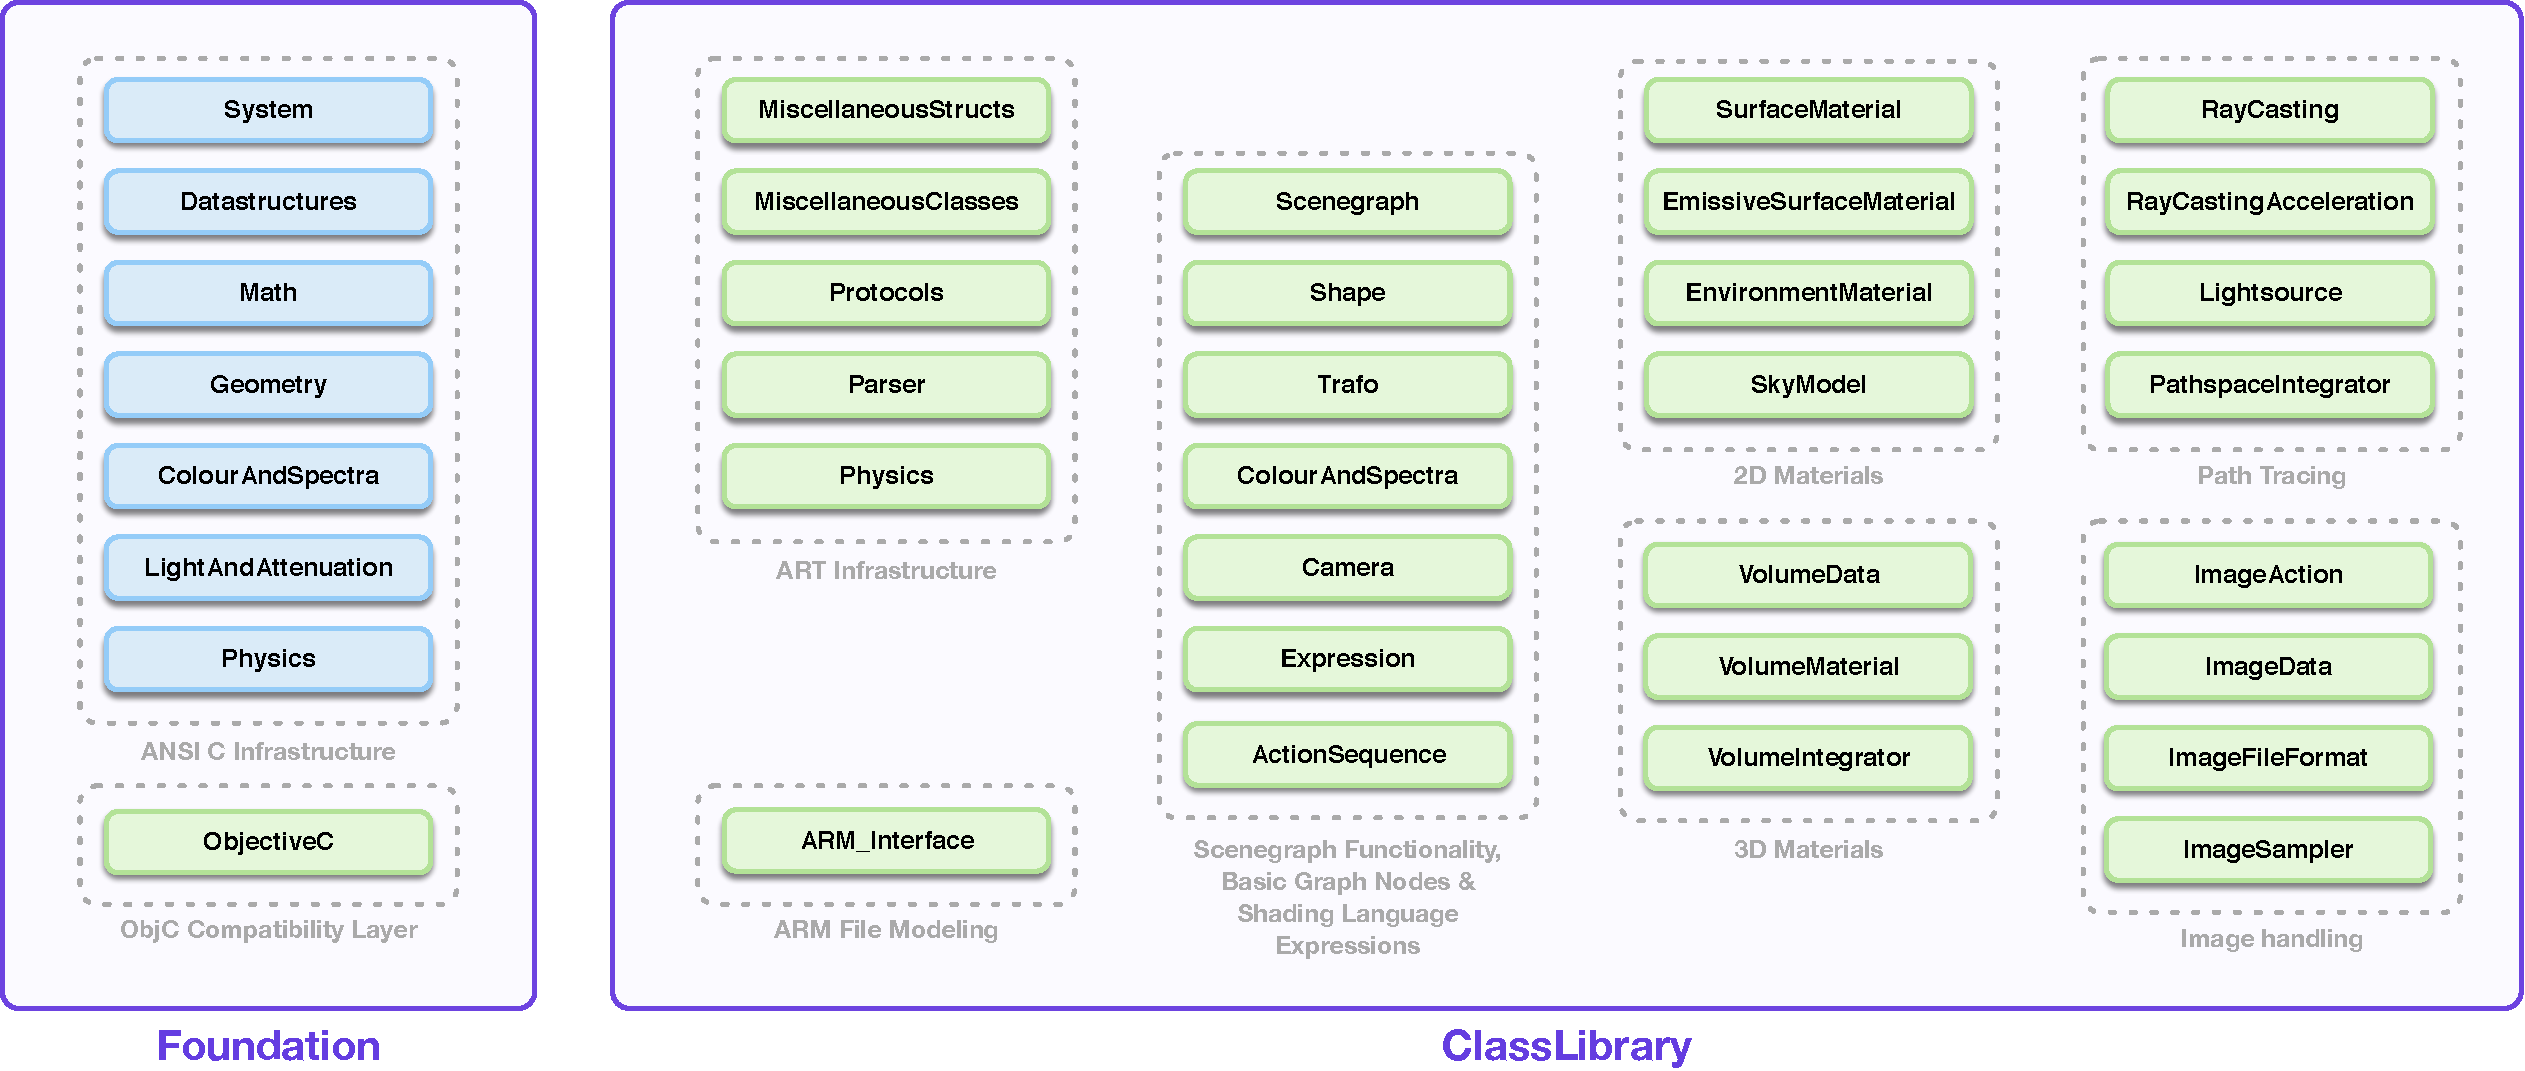
\includegraphics[width=.99\linewidth]{Images/ART_Library_Structure.pdf} 
\end{center}
\caption{
\label{fig:librarystructure} 
The overall internal structure of the ART library. Blue boxes signify sub-directories with ANSI C code, green boxes stand for Objective-C code. Note that two directory names (\source{Physics} and \source{ColourAndSpectra}) occur in both \source{Foundation} and \source{ClassLibrary}: the \source{Foundation} version contains simpler, pure ANSI C code, while the \source{ClassLibrary} directory contains classes that offer higher-level functionality. For instance, \source{ColourAndSpectra} in \source{ClassLibrary} contains scene graph nodes that deal with spectra and colours, while the 
\source{Foundation} equivalent provides low-level data types.}
\end{figure}

\subsection{Individual Source Files as \emph{ART Modules}}

Each compiled source file within ART (\ie each \source{.c}, \source{.m} or \source{.mm} file) is treated as a \emph{module}, which can have its own global state that is initialised when ART is started up, and which is destroyed in an orderly fashion when ART is shut down. To this effect, all modules contain a startup and a shutdown function, which are defined in a way that is intended to be as unobtrusive as possible. To give an example, the file \source{Foundation/System/ArTime.h} contains the following line, right after the copyright header:

\begin{verbatim}
ART_MODULE_INTERFACE(ArTime)
\end{verbatim}

This line is all that is needed for defining the appropriate function prototypes for starting and shutting down the \source{ArTime} module. In the corresponding source file \source{ArTime.c}, the following lines are also placed right at the beginning:

\begin{verbatim}
#define ART_MODULE_NAME     ArTime

#include "ArTime.h"

ART_NO_MODULE_INITIALISATION_FUNCTION_NECESSARY

ART_NO_MODULE_SHUTDOWN_FUNCTION_NECESSARY
\end{verbatim}

These lines define empty startup and shutdown functions: even if a particular source file does not need any global state, these empty functions should always be placed at the start of the source file in question. The cost of calling one empty function per source file in ART during startup is negligible, and systematically providing all modules with these functions ensures that one has module startup/shutdown infrastructure available in all parts of the system, if it were needed at a later stage in development.

Each "library" (\ie grouping of source files into thematically related source file directories, see above) has the responsibility to call the startup functions for all modules in the directory: this means that one has to manually add an appropriate line to the corresponding startup function of the library when one adds a new source file to a given directory. This is not a frequent operation, so this overhead was deemed permissible. These library startup modules are canonically named, and easy to identify: an example would be 

\begin{verbatim}
ART_Foundation_Math.[h|c]
\end{verbatim}

\subsection{Module State: the Ubiquitous Variable \source{art\_gv} }

The entire ART system is written in a way that it does not depend on any truly global variables. But as any rendering system of such size has some state associated with it, there is a ubiquitous reference within the entire codebase to something we refer to as the \emph{"ART Global Variables"}, or \source{art\_gv} for short. The data type of this variable is \source{struct ART\_GV}, and it is defined in \filename{Foundation/System/ART\_GV.h}. It is the top-level location where during module startup (see previous section), any ART module can store variable information that has to be globally accessible for a given, running instance of ART.

Apart from this struct, there are no genuine global \emph{variables} in ART, only global \emph{constants}\footnote{Some global constants, such as the \source{CRC32} tables, are actually defined as variables for technical reasons. These should never be modified, but they are usually protected by being encapsulated in their modules anyway.}. Two instances of ART can cleanly co-exist in the same memory space if each of them has their own copy of this global variable struct, and this also ensures that ART can be safely run from/as a shared library, irrespective of the memory/linkage model which is used.

There is exactly one instance of type \source{struct ART\_GV} for each running ART instance, the components of which are successively initialised during the library and module initialisation phase, and de-activated in reverse order during module shutdown. The only functions that are allowed to create the components of this struct are the canonical module startup functions discussed in the previous section, and the only ones who are allowed (and expected) to destroy its contents are the corresponding canonical module shutdown functions.

The actual data type of individual \source{art\_gv} entries is defined in each of the modules, so that no modules in ART can actually see the contents of other module \source{art\_gv} entries.

\subsection{Starting Up ART, and Shutting It Down Again}

When starting up an ART command line application, it is important that the various background sub-systems, such as the module system discussed in the preceding sections, but also the command line option handling, are started up and shut down in an orderly fashion. To make this as unobtrusive as possible, ART applications do not define their own \source{main()} functions, but instead use a template (shown here for the \source{artist} rendering application) somewhere at the end of the main source file:

\begin{verbatim}
ADVANCED_RENDERING_TOOLKIT_MAIN(artist)
\end{verbatim}

This macro defines the actual \source{main()} function called on application start-up: the predefined function takes care of all startup and shutdown issues necessary for proper ART operation. Centrepiece of this function is that it calls a user-defined actual \source{main()} function of the application, which has to have the supplied name. This function also has to have exactly the function signature seen in this example.

\begin{verbatim}
int artist(
        int        argc,
        char    ** argv,
        ART_GV   * art_gv
        )
{ ...actual code of the executable goes here... }
\end{verbatim}

Note that this signature is the same as that of a normal UNIX \source{main()} function, plus a pointer to a properly initialised \source{art\_gv} instance. This pointer is transparently passed on to all instances of Objective-C objects in the system: all classes in ART are derived from \class{ArcObject}, which contains a reference to \source{art\_gv}. As instances of \class{ArcObject} are only created via special macros which require \source{art\_gv} to be defined, the pointer is transparently passed on to all derived instances.

\section{ART as a Mixture of ANSI C and Objective-C}
\label{sect:mixingCandC}

A rather specific feature of ART which has been around since the very beginning of the 0.x series is the split of the system into a low-level ANSI C part, and a high-level Objective-C part. Unlike C++, which superficially looks a lot like C, but is actually a separate language, Objective-C is a strict superset of ANSI C, and the two can be freely intermixed and crosslinked. Back when the first versions of ART were designed by Robert F. Tobler, he carefully analysed the run-time behaviour of Objective-C, and came up with an initial distribution of data types into low level C structures, and high level ObjC classes. It is a testament to the quality of his work that this global design did not have to be modified a lot since then.

Even more than 20 years later, this split makes sense, given the properties of Objective-C: it is a powerful object-oriented language, and its advanced features such as introspection are provided via a run-time system. However, partly due to the overhead of the run-time system, one should avoid use of ObjC classes in the innermost loops of computation-intensive tasks -- at least if the instances in question might get frequently created, destroyed or modified there. In these cases, use of carefully managed ANSI C structures mani\-pulated via plain C functions make more sense, performance-wise. 

This means that in a renderer, it is reasonable to use ObjC for high-level semantic descriptions, such as the scene graph: but to also use C for low-level constructs such as points, vectors, spectra, or RGB colour values. As a consequence, the low-level libraries -- i.e. all those in \command{ART\_Foundation}, with the exception of \command{ART\_Foundation\_Objective} -- are written entirely in ANSI C99, and Objective-C is employed only \emph{above} those. However, even in high-level libraries one can find plenty of plain C structures in places where they are needed, again mostly for performance reasons.

%%%%%%%%%%%%%%%%%%%%%%%%%%%%%%%%%%%%%%%%%%%%%%%%%%%%%%%%%%%%%%%%%%%%%%%%%%%%%%%%%%%%%%%%%%%

\chapter{Memory Management in ART}
\label{sec:ARTmemorymanagement}
In this chapter, the memory management approach used on the data structure \&~class level within ART is explained. There are two main approaches to manage object persistence in non-trivial software systems:
\begin{enumerate}
\item \textbf{Garbage Collection} \\ \textit{Key advantage}: very resilient against memory-related programming errors, since no large-scale adaptation of the software is necessary. \\ \textit{Key disadvantages}: there is always a run-time penalty for the collection cycles, and if tight inner loops allocate large amounts of instances in short periods of time, memory usage spikes may result. Running the garbage collection more often to avoid such spikes reduces performance even further. Also, such usage spikes may not even be properly predictable in the first place.
\item \textbf{Reference Counting} \\ \textit{Key advantages}: memory usage never exceeds the actually needed amount, and no garbage collection cycle times are introduced. \\ \textit{Key disadvantages}: the entire software architecture has to be adapted, and it is fairly easy to make subtle and hard to find coding mistakes.
\end{enumerate}

Many years ago when the basic software design of ART 0.x was defined, reference counting was chosen as the memory management model. That was in 1996, when no robust drop-in garbage collectors existed yet, so there was little alternative to doing it this way. When the ART 2.x effort was started, it was intended to be, as far as possible, a gradual evolution and stabilisation of the ART 1.x codebase. But even fundamental design decisions like the memory management strategy were reconsidered -- especially since viable garbage collectors had become available in the meantime. 

There main reason why ART 2.x, after careful consideration, stayed with the reference counting approach of ART 1.x (albeit in an almost completely re-designed fashion) was that the potential performance penalty and memory overhead incurred by using garbage collection was deemed as being too much of a risk. In a rendering toolkit which features a shading language that is not statically "baked" into the terminal objects in a pre-processing pass (which we cannot do, as we do not break down the scene into micro-polygons before rendering), scene graph traversals can, under certain circumstances, create and almost instantly discard lots of small temporary object instances within very short timeframes. This is one usage case where garbage collection just will not work properly.

As already mentioned, the reference counting mechanisms in ART~2.x were significantly altered compared to ART~1.x. In ART~1.x, these mechanisms were not strongly formalised, somewhat varied in their semantics between different classes, and proved to be a persistent source of instability in the entire toolkit throughout its lifetime. Therefore, ART~2.x uses a fairly rigid and unified approach how object references are handled: these guidelines are what is described in the following sections of this chapter. 

\section{Design Goals of the ART Memory Management}

Those experienced in Apple MacOS application development will notice that our approach deviates to some degree from Objective-C memory management guidelines provided by Apple: ART reference counting is slightly more complicated than what MacOS does, and uses a functionality extension that is specific to ART. The extension was unfortunately necessary since ART has different goals, and faces different constraints, than the normal multi-purpose Cocoa software frameworks used for MacOS and iOS application programming. In particular, within ART object reference handling faces the following additional constraints: 
\begin{enumerate}
\item The main difference between ART and standard Cocoa/GNUStep programming is that the ability to achieve \textbf{lock-free parallelism between large numbers of rendering threads} is much more important for us than it is for normal OS~X/iOS application programming. We \textit{need} to be able to run one rendering thread per core (of which there are hopefully many), with no locking synchronisation between them taking place \textit{at all}.
\item Since descriptions of scene geometry, and their associated ray intersection acceleration structures such as kD-trees, can be very large, these many rendering threads all have to share a single copy of the scene database. By extension, this means that the rendering threads can not use retain/release operations (\ie the cornerstones of normal NSObject memory management) on that shared scene description: such operations are either not threadsafe, or -- with the OS~X/iOS runtime switched to multi-threaded mode -- use an internal semaphore protection on the reference counters that completely sends multi-thread performance down the drain.
\item Points 1 and 2 have the consequence that we have to \textbf{override the native retain/release mechanism of NSObject} with something of our own devising. The reason for this is that we still have to invoke release/retain on some objects during rendering. Since ART is designed so all these retain/release operations take place only within individual rendering threads, we do not need or want the semaphore protection that the native NSObject retain/release enforces once the system goes into multi-threaded mode.
\item During the rendering process, the presence of shading language functionality means that certain object properties, such as surface reflectance, can either be provided by actual scene database nodes (if no SL constructs are being used), or by a temporary object that contains the SL evaluation result for a particular ray-object intersection. This temporary object has to be discarded after use, while the actual scene database node must not be altered.
\item The previous point means that we need the capability to \textbf{distinguish between weak and hard object references} that are being passed to calling functions. In some cases, object references have to contain information on whether the caller should take ownership of the object it receives (in the case of a temporary node which the receiver will need to discard after use), or not (if an actual scene graph node is returned, which should not be released).
\end{enumerate}

\section{ART Memory Management - Used Data Structures}

References to object instances are normally pointers - and in ART, this is of course also the standard data type to use. Across ART, some pointers are retained by the caller, some not: which strategy applies to any given pointer should be obvious from the class definition (\ie the comments in the class definition should clearly say, for each and every pointer, to which category it belongs).

However, there are also two data types that are intended to replace pointer references to object instances in ART class definitions in all those cases where a pointer could, depending on context, be either a weak or a hard link. These types are \textbf{\filename{ArObjRef}} and \textbf{\filename{ArNodeRef}}. Apart from the typing of their contents (\filename{ArcObject} \vs \filename{ArNode} pointers), these structs are identical, and contain two fields: the pointer to the instance in question, and a field that determines whether the reference is a weak or hard link. Hard and weak references to a node instance are created by the macros \filename{HARD\_NODE\_REFERENCE(<pointer>)} and  \filename{WEAK\_NODE\_REFERENCE(<pointer>)}. The node instance pointer contained in an \filename{ArObjRef} can be accessed via \filename{ARNODEREF\_POINTER(<objref>)}.

\section{ART Memory Management - Usage Rules}

The following rules apply to all classes that are implemented within ART. (ToDo: gather the appropriate info from various header files in the source tree, where it is already provided)

%%%%%%%%%%%%%%%%%%%%%%%%%%%%%%%%%%%%%%%%%%%%%%%%%%%%%%%%%%%%%%%%%%%%%%%%%%%%%%%%%%%%%%%%%%%

\chapter{Scene File Formats}
\label{sec:scenefileformats}

In this section, we refer to all types of input files used to drive rendering jobs as "scene files", even if they only cover one particular aspect of scene appearance, or rendering behaviour. The only exception are image file formats, which are discussed in the next section.

\section{Proprietary Scene File Formats}

\begin{description}
\item[\filename{.arm}]: the native Objective-C scene file format of ART. This is the master scene file format used to drive all rendering jobs. These files are actually valid Objective-C code which constructs the scene in question, and are compiled and run in order to yield parseable \filename{.art} files: see section~\ref{sec:ARTscenefileformat} for details about how this format is read and handled by the toolkit. The extension \filename{.arm} is derived from the general prefix of things in ART (\filename{Ar...}), plus the letter \filename{m}. Normal Objective-C source files use the extension \filename{.m}, and as \filename{.arm} files contain valid Objective-C code, the combined extension makes sense.

\item[\filename{.art} / \filename{.arb}]: the internal storage format of native scene files. These are not intended to be manually edited, and their relationship to \filename{.arm} files is explained in section~\ref{sec:ARTscenefileformat}.

\item[\filename{.arh}]: ART resource header files. These are regular Objective-C header files that are used for library functions within the ART resource pool that is provided with the system. Changing the extension of these files to \filename{.h} makes no difference to their functionality, and putting resource data into regular header files would also work. The proprietary extension only serves to distinguish purely \filename{.arm}-file related headers from normal Objective-C headers.

\item[\filename{.ark}] files. These are measurement archives that usually contain spectral measurement data for reflective surfaces, and other physical measurements of materials. The archive files are intentionally human-readable, intentionally quite verbose, and the actual measurement data is stored in a format that allows direct copy and paste to Mathematica notebooks for visualisation purposes.

\end{description}

\label{sect:propsceneformats}
\section{Standard Scene File Formats}
\label{sect:stdsceneformats}

\begin{description}
\item[\filename{.ply}]: 3D mesh data. PLY is a computer file format known as the Polygon File Format or the Stanford Triangle Format. ART is capable of parsing such files, and including the geometry defined by them in native ART scenes. Support for such meshes is still not 100\% stable, unfortunately: in a few rare instances, the kD-tree builder can fail for highly complex models. Also, no mapping between vertex attributes and ART surface and material descriptors is possible yet. Currently, one can only assign one surface and one material node to the entire object described by a PLY mesh.


\end{description}

\section{Internal Handling of ARM Files}
\label{sec:ARTscenefileformat}

An at first glance perhaps slightly peculiar feature of ART is that it is actually not able to directly parse its native scene description language: the
Objective-C based \command{.arm} format. 

Instead, the native file formats that ART is actually capable of parsing are the \command{.art} and \command{.arb} formats, respectively. These two are basically the same format,
with \command{.art} being a still human-readable ASCII form of a linearised scene
graph encoding with absolute references that can easily be parsed, and
\command{.arb} being a diskspace-saving binary version of exactly the same
format. There is also a utility called \command{arb2art} available to convert
\command{.art} files to \command{.arb} format and back.

Note that \command{.art} files are -- while being intentionally
human-readable -- not really intended to be edited; although minor changes
(such as to numerical parameters of a node) can be made, any major
changes require prohibitive effort due to the absolute nature of the
references.

The \command{.arm} format is actually plain Objective-C -- the
object-oriented dialect of ANSI C in which ART itself is written. This
offers all the flexibility and power of being able to write full
C/Objective-C programs which generate the objects in the scene, and takes the
burden of maintaining such a powerful parser off the project, since
\command{gcc} or \command{llvm} are used for the translation.

Side note: by design, \command{.art} files are actually a special form of quine. The human readable form of the linearised scene graph was defined so that it is also valid Objective-C, and that it is in the right arrangement for actually even being a valid \command{.arm} file. Change the extension of any \command{.art} file back to \filename{.arm}, and you can translate it to \command{.art} form again using \command{arm2art}. Which is of course pointless, but in a certain way, also beautiful. :) Credit for this particular feature goes to Robert F. Tobler, the lead designer of ART 0.x and 1.x. We recall him enjoying himself immensely while coming up with this idea.

\subsection{\command{.arm} File Structure}
Apart from the fact that they have to be valid Objective-C, there is only one
constraint which \command{.arm} files have to fulfill in order to be usable by
the toolkit. They have to contain at least one C function with a canonical name and form:
\begin{verbatim}
ARM_MAIN_FUNCTION(<filename minus the .arm>)
{
    //   construction/initialisation of the scene object goes here
    
    return <scene_object>;   // <- return the completed scene 
                             //    object that was created
}
\end{verbatim}
so that e.g.\ the file \filename{ToyEngine.arm} has to contain a function called
\begin{verbatim}
ARM_MAIN_FUNCTION(ToyEngine)
{
    ...
}
\end{verbatim}
This "main" function has to return an \filename{ArnScene} object that defines the
overall scene structure -- see section~\ref{sec:usingart}, \emph{Using ART}, for an explanation of
its significance. Apart from this, anything goes with respect to the contents of the file. In particular, the file may include arbitrarily many other files, define functions, and do anything else that Objective-C allows. In the directory \filename{ART/Gallery}, a number of example files are provided: inspecting these will quickly give you an idea how all this works in practice.

Also, the separate "ARM Scene File Interface" guide provided in the \filename{ART/Documentation} directory gives a detailed overview of \source{.arm} file options and structure.

\subsection{Translation of \filename{.arm} to \filename{.art}}

Translation of \filename{.arm} to \filename{.art} files is simple. It is either
performed automatically in the background via a forked sub-process by \filename{artist} (or any other ART executable) whenever it senses the associated \filename{.arm} file to be newer than the corresponding \filename{.art} file, or by explicitly calling the command
\command{arm2art} as in
\begin{verbatim}
arm2art foo.arm
\end{verbatim}
or for a binary \filename{.arb} result file
\begin{verbatim}
arm2art -b foo.arm
\end{verbatim}

The actual "conversion" between \filename{.arm} and \filename{.art} is a bit of a hack, but harmless. 

First, the name of the main function of the top level \filename{.arm} file is fixed via an in-place editing pass done with \filename{sed}. This is a convenience for the end user: the requirement that the main function in a file called \filename{<filename>.arm} has to be named \filename{ARM\_MAIN\_FUNCTION(<filename>)} would make \filename{.arm} files brittle against name changes done from the command line: if you re-name an existing \filename{.arm} file, the name of the main function has to change as well. Having to do this manually every time you re-name an \filename{.arm} file would be a hassle, so the sed pass makes sure the \filename{ARM\_MAIN\_FUNCTION()} matches the filename. 

After this, the actual translation happens. In the \filename{ART\_Resources/arm2art} directory a file named \filename{ArtTranslationStub.m} is provided. What the conversion process does is the following: the scene file in question is \filename{\#included} in the stub source, the stub compiled, and the resulting executable is then run. The stub only contains a simple main routine which calls an
\filename{ArnScene}-generating function for the scene source file (the one called \filename{ARM\_MAIN\_FUNCTION(<filename minus the .arm>)}), and then simply saves this newly generated
scene graph to disk using the internal \filename{.art} format writing
routine. As last step, the translation process removes the executable which was generated to write the \filename{.art} file.


%%%%%%%%%%%%%%%%%%%%%%%%%%%%%%%%%%%%%%%%%%%%%%%%%%%%%%%%%%%%%%%%%%%%%%%%%%%%%%%%%%%%%%%%%%%

\chapter{Image File Formats used by ART}
ART uses two kinds of image formats: proprietary -- but documented -- ones for
intermediate storage of rendering results, and mainstream types for
general output.
\section{Proprietary Image File Formats}
\label{sect:propformats}
A spectral rendering system like ART has to have the capability to save the results of its
computations in a lossless intermediate format. Since ART is a rendering system that is
capable of handling spectral radiance information, and optionally also the polarisation
state of light, using existing image formats for this purpose
was unfortunately not an option. While there are multispectral some image formats out there -- mainly for use in astronomy, e.g.\ FITS -- these were designed with such different goals in mind than
fulfilling the needs of a photorealistic rendering system that it proved simpler
to design our own formats.

There are three intermediate formats specific to ART: \filename{artraw}, \filename{artcsp}
and \filename{artgsc}. The three have the following purposes: \filename{artraw} is used to
directly store all the raw information provided by the renderer which was called
by the user (which might be spectral data -- possibly including polarisation
information -- or simple colourspace values) without performing any compression, \filename{artcsp} always stores -- also uncompressed -- \filename{CIE XYZ}
colour values, while \filename{artgsc} stores single channel float images.

\begin{description}
\item[\filename{artraw}] The first format -- files with extension
    \filename{.artraw} -- has the purpose to retain all information
    available from the rendering pass, and can therefore have a wide
    variety of contents. This has to be read and interpreted by ART in any of the ISR modes it can be switched to (see section~\ref{sect:CCTs}), so the
    image format code has a crossbar-switch quality to it that makes
    it pretty specific for its purpose. An RGB renderer or tonemapper
    \eg has to be capable of interpreting a polarised spectral image
    (by converting the values to colour space and discarding the
    polarisation information), just as a polarisation-aware executable
    has to be able to read \eg \filename{CIE XYZ} image data (by
    performing an -- intrinsically problematic -- construction of
    spectra for the colour values).
    
  \item[\filename{artcsp}] The second format -- files with the
    extension \filename{.artcsp} -- is much simpler (no crossbar
    functionality -- the code is comparatively straightforward), since
    it just reads and writes floating-point colour values. It became
    necessary to develop this once we realised that prior to the availability of OpenEXR, all high-dynamic range colourspace
    formats we have been able to include in ART up to that point apparently
    performed some kind of lossy compression. Small as the error
    introduced by that was in most cases, we managed to find some
    where it made a difference. This format could be obsoleted once a
    lossless HDR format has been included in the toolkit, which now arguably is the case with OpenEXR. But then, we might just leave it in place -- never touch a running system, and \filename{artcsp}
    is used purely for internal purposes anyway. Also, in its default mode, OpenEXR tends to cut off numerically tiny result values, which has bitten us in the past.

  \item[\filename{artgsc}] The third format -- files with the
    extension \filename{.artgsc} -- is even simpler than \filename{.artcsp}: it only contains a single channel of intensity values. The reason for its existence is quite similar to why \filename{.artcsp} was created: and it is separate from \filename{.artcsp} so that a simple differentiation what kind of content what can expect is possible at the filetype level.

\end{description}
None of the three formats performs any compression, since image file size is usually not an issue for single intermediate images, and the user is free to run
\command{gzip}, \command{bzip} or some other compression tool of their choice
(which is in all probability more efficient than the kind of format-specific
lossless compression scheme we could come up with anyway) on the files if they
want to retain them.

The internals of all three formats are documented at the beginning of the
implementation files for their file format classes in:
\filename{ArfARTRAW.m}, \filename{ArfARTCSP.m} and
\filename{ArfARTGSC.m},
respectively.

\section{Standard Image File Formats}
These are used both as input formats for 2D textures (imagemaps) and as final
output formats for displayable results of rendering or tone mapping jobs. They
unfortunately differ with respect to the quality of their support in ART;
limitations are discussed along with each format.

\begin{description}
\item[Standard TIFF] Read/write implemented through Sam Leffler's TIFF
  library. Works flawlessly, and is the standard format for providing
  RGB output.
\item[JPEG] Only reading is implemented. The intention behind this was
  that lossy compression of result images is best done elsewhere, but
  that the renderer ought to be able to read JPEG imagemaps. Support is optional, and contingent on \filename{cmake} finding the JPEG library during set-up.
\item[OpenEXR] Read/write support implemented. Support is an optional feature, though: it is only present if \filename{cmake} finds the OpenEXR library during the set-up phase.
\end{description}

%%%%%%%%%%%%%%%%%%%%%%%%%%%%%%%%%%%%%%%%%%%%%%%%%%%%%%%%%%%%%%%%%%%%%%%%%%%%%%%%%%%%%%%%%%%

\chapter{Input Handling  --  File Format Handling Classes}
\label{sec:Background:InputHandling}

ART uses a modular approach to file formats. Any input data type which
can be read from file -- be that images, reflectance measurements,
scene graphs, action sequences, \ldots -- is represented by a so-called
\emph{file format handling class}. The main task of these
classes -- the names of which always begin with \class{Arf\ldots}, e.g.
\class{ArfTIFF} -- is to parse a given file, and to construct an
appropriate ART-specific representation in memory for its contents.

During application initialisation all such classes have to register
themselves with the so-called \emph{file probe} class (see the source
of an \class{Arf\ldots} class for an example of this -- the
\filename{Image} library is a good place to start looking), which is
responsible for the selection of the correct format handling class for
a given file. Amongst other things, each \class{Arf\ldots} class can
specify a list of file extensions for which it feels responsible, and
is only queried further if the filename matches one of them.

When reading a file from disc, all the programmer ever does is to request
parsing of a file which he identifies by name, and if any of the ART format
handling classes can make sense of the file contents (the file probe class holds
a contest amongst all registered format handlers to find the best one) he
receives an object instance in return:
\begin{verbatim}
object =
    parse_file(
        art_gv,
        inputFileName,
        includeLibraryPathInSearch
        );
\end{verbatim}
Due to the polymorphic nature of the parse process this \variable{object} can
theoretically be any of a wide variety of types; if the file contained a
\filename{JPEG} image, the resulting instance is actually an image
representation, while an \filename{.arm} file would result in a scene graph
object. Consequently, care has to be exercised that the correct kind of file is
parsed at the right time, and clean programming in ART would require that
objects which are read from disk are queried whether they conform to the
protocols which are needed by the calling application afterwards. 

For instance, in a scenario where the \var{object} parsed in the previous
example is expected to be an image, such a check would be achieved by the
following code: 
\begin{verbatim}
if ( [ object conformsToArProtocol: ARPROTOCOL(ArpImage) ] )
    <do whatever you intended to do>
else
    <complain / raise an exception / whatever> 
\end{verbatim}

%%%%%%%%%%%%%%%%%%%%%%%%%%%%%%%%%%%%%%%%%%%%%%%%%%%%%%%%%%%%%%%%%%%%%%%%%%%%%%%%%%%%%%%%%%%

\chapter{ART Naming Conventions}
\label{sec:Background:Naming}
For a large project like ART a consistent naming scheme for the entities which
make up the data structures within the code is crucial. Here we outline the basic
rules according to which the canonical names for structures, classes and similar
entities are derived.

\section{Data Types}
The ART libraries define a large number of data types which fall into different
categories -- C structures and several subtypes of Objective-C classes. Since
there are examples of similarly named entities which fall into different
categories, a partitioning of the project namespace according to this category
was deemed a sensible move.

Note that all data types in ART start with capital letters and are mixed case,
e.g. \class{Pnt3D}, \class{ArnSphere}  or
\class{ArnPathTracer}. Table~\ref{tab:datatypes} lists the existing
categories.

\begin{table}[htbp]
\centering
\begin{tabular}{|l|l|p{2.2cm}|p{5.7cm}|}
\hline
\textbf{\textit{Form}} 
& \textbf{\textit{Type}} 
& \textbf{\textit{Examples}} 
& \textbf{\textit{Comments, Exceptions}} \\ \hline

\class{Ar\ldots}
&
C structures and C enumerations
&
\class{ArLight} \newline
\class{ArMesh} \newline
\class{ArFileMatch}
& 
A few C structs do not follow this scheme, \eg \class{Pnt3D}. Most offenders 
   are from the \class{Graphics} library: \class{ArPnt3D} sounded too elaborate.

Sole exception in the other direction: \class{ArNode} is a node class, not a C struct (\class{ArnNode} sounds wrong) \\ \hline

\class{Arp\ldots}
& Objective-C protocols
& \class{ArpShape} \newline
\class{ArpLightsource}
& The equivalent to Java interfaces. \\ \hline

\class{Arc\ldots}
& Generic Objective-C classes
& \class{ArcRandom}
& Plain objects which are not intended to be part of scene graphs, and which are neither saved to nor
  read from file like scene graph nodes are. \\ \hline

\class{Arf\ldots}
& File format handling class
& \class{ArfTIFF} \newline
\class{ArfARTRAW}
& \class{ArcObject}-derived classes for file handling. \\ \hline

\class{Arn\ldots}
& Scene graph classes
& \class{ArnSphere} \newline
\class{ArnPathTracer}
& Nodes are the building blocks for
  scene graphs. These can be read from, and saved to, ART scene files.\\ \hline

\class{Ara\ldots}
& Scene graph attribute classes
& \class{AraTrafo3D}
& A special kind of node: all such node classes contain an indirection to an object property (shaders, trafos, \etc). Apart from this, they are normal scene graph nodes. \\ \hline

\end{tabular}
\caption{Schematic of data type naming in the ART libraries.}
\label{tab:datatypes}
\end{table}

\section{Enumeration Types}
C enumerations follow the same naming convention as C structures, namely that
they have to be of the form \class{Ar<name>}. The actual entries of the enum
are all lowercase, and their names are of the form:
\begin{verbatim}
<enum name in lowercase>_<actual value name>
\end{verbatim}
A typical example for this would be the return type of file type matching
operations:
\begin{verbatim}
typedef enum ArFileMatch
{
    arfilematch_impossible = 0,
    arfilematch_possible   = 1,
    arfilematch_exact      = 2
}
ArFileMatch;
\end{verbatim}

\chapter{Surface Materials \vs Volume Materials}
\label{sec:SurfacesVsMaterials}

In order to facilitate physics-based modelling, ART makes the usual distinction between \emph{surface materials} (\ie BRDF models), and \emph{volume materials} (which cover both material properties, and volume effects). There are a few non-standard aspects to how ART treats the relationship between those, which get explained here.

\begin{figure}[htbp]
\begin{center}
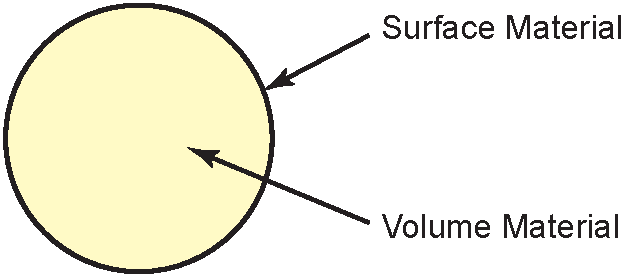
\includegraphics[width=.3\linewidth]{Images/SurfaceVsMaterial.pdf} 
\end{center}
\caption{
\label{fig:surfacevsmaterial} 
Relationship between the \source{Surface Material} and \source{Volume Material} attributes of a shape. The surface material describes the behaviour of light at the phase boundary between the shape and its surroundings. The volume material model describes both the physical properties of the volume (such as its refractive index relative to vacuum), as well as providing a mathematical model for the interaction of light with the volume inside the object.
}
\end{figure}

In other rendering systems, the mathematical models for light-surface interactions are referred to via a number of equivalent names: \emph{surface shaders}, \emph{BRDF models}, \emph{reflectance models}, and sometimes also \emph{shading models} or even \emph{illumination models}. Arguably, from a physics viewpoint, the last name in this list borders on being misleading, as these models still primarily deal with the properties of the surface in question, and not the incident illumination as such. But the expression is still common in real-time graphics.

In addition to descriptions of surface reflectance, most rendering systems also feature models for the interaction of light with volumes. These are referred to as \emph{volume shaders} or \emph{scattering models}, and are usually handled separately from the physical attributes (such as the index of refraction, or the volumetric absorption coefficient) of the objects in the scene.

In ART, we attempt to take a more unified view on this, in that each object in the scene is assumed to have a \emph{volume material} which describes its physical material properties, and, by extension, also the interaction of light with its volume. A motivation for this is that these two aspects of appearance are often tightly connected. On the other hand, the \emph{surface models} in ART are used as descriptors of light-matter interactions at phase boundaries, \ie~at the surfaces of objects. Figure~\ref{fig:surfacevsmaterial} illustrates this concept. 

This design allows for intuitive modelling insofar as surface models can take those of their input parameters which depend on the physical properties of the object they are applied to from the material description of that object, and do not have to store them themselves. An example of this are Fresnel surfaces: the main parameter of such a BRDF is the refractive index at the phase boundary. But the Fresnel surface class does not, by default, store an index of refraction, but rather uses the IOR found at the phase boundary it is being applied to instead. 

\begin{figure}[htbp]
\begin{center}
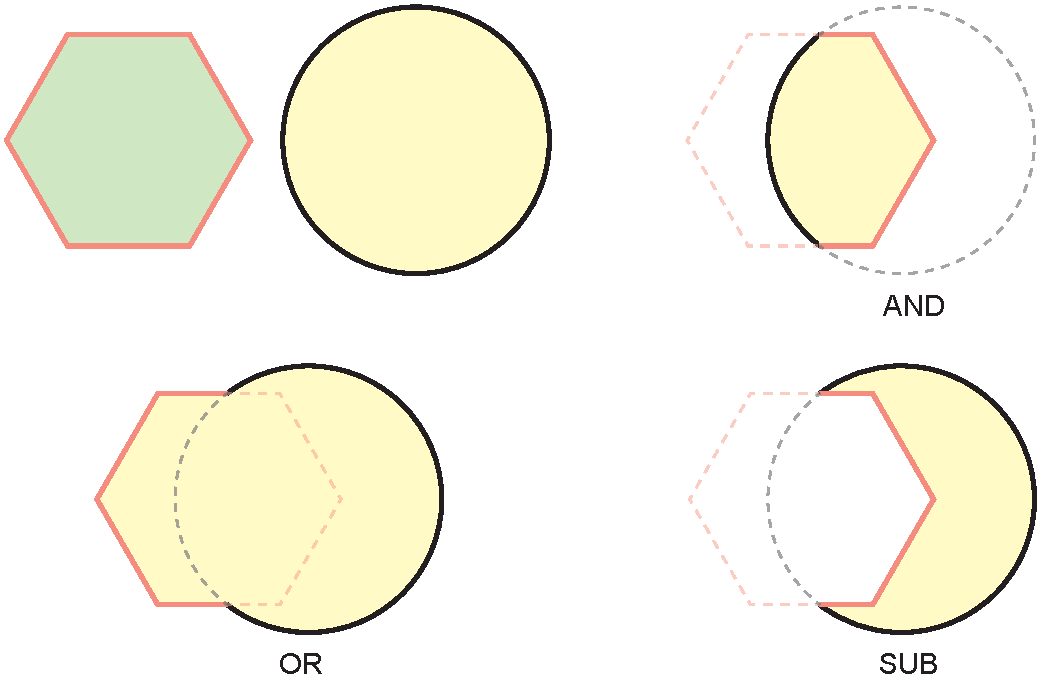
\includegraphics[width=.5\linewidth]{Images/SurfaceVsMaterialCSG.pdf} 
\end{center}
\caption{
\label{fig:surfacevsmaterialCSG} 
Behaviour of surface and volume material attributes during CSG operations. Here, it is assumed that the yellow sphere has precedence over the green hexagon, so its material is applied to the entire result. In ART, the first argument of a CSG operation has precedence over the second one, so in an \source{.arm} file, the corresponding command would \eg be \source{[sphere~sub:~hexagon]}. Note that if the red surface originally applied to the green hexagon is a BRDF which depends on volume material properties (such as a Fresnel surface material, which uses the IOR of the underlying volume material), it will use the IOR of the yellow volume material on the CSG objects! This behaviour can \eg be used to cut a piece from a glass sphere painted with opaque paint, so that one sees the glass inside again.
}
\end{figure}


From a modelling perspective, these are arguably fairly intuitive semantics for describing objects that have volume: if an object is considered to be made of glass, it has to have a glass material that, apart from storing the index of refraction of the particular type of glass used, also defines how light is attenuated inside the object (\ie also stores the transmission colour of the glass). And if the BRDF which is applied to this object needs to make use of some of this information such as the IOR, the surface model queries the material attribute for this data. 

However, an opaque BRDF which ignores the material properties can still be applied to such a glass object -- semantically, this would correspond to a glass object \eg being painted with a layer of lacquer. Inside, the object is still made of glass, though, and if CSG operations are used to cut pieces from the sphere, the glass again becomes visible. See figure~\ref{fig:surfacevsmaterialCSG} for an illustration of CSG semantics with respect to materials and surfaces.

\chapter{Surfaces}
\label{sec:Surfaces}

In this chapter, we describe some of the the technical background of the implementation and evaluation of BRDF models in ART, and present a list of the implemented models. 

\section{Technical Background}

At the moment, this section mainly focuses on things that ART does in a non-standard way, or on those aspects of a renderer where no widely accepted solution exists, and where the particular technique used in ART is worth discussing. Therefore, this section is not a complete introduction into BRDFs and surface rendering.

\subsection{The ART BRDF Model Coordinate System}
In CG literature, BRDF models are usually defined for a local coordinate system with normalised vectors of unit length that all point away from the location at which the BRDF is evaluated, and that have certain canonical names. A graphical overview of this notation is shown in figure~\ref{fig:LiteratureSurfaceCoordinateSystem}.

\begin{figure}[htbp]\centering
  \setlength{\unitlength}{2mm}
  \begin{picture}(25,10)(-10,0)
      \put(-10,0){\line(1,0){20}} % baseline
      \put(0,0){\vector(0,1){10}}     \put(0,10){$\vec{N}$} % N
      \put(0,0){\vector(-1,1){7.071}} \put(-7.071,7.071){$\vec{L}$} % L
      \put(0,0){\vector(1,1){7.071}}  \put(7.071,7.071){$\vec{R}$} % R
      \put(0,0){\vector(1,6){1.6}}    \put(1.6,9.87){$\vec{H}$} % H
      \put(0,0){\vector(2,1){8.944}}  \put(8.944,4.472){$\vec{V}$} % V
    \end{picture}
\begin{tabular}[b]{lll}
$\vec{n}$        &$\vec{N}$& surface normal \\
$\vec{\omega_o}$ &$\vec{V},\vec{E}$& outgoing direction (``eye'', ``view'') \\
$\vec{\omega_i}$ &$\vec{L}$& incoming (``light'') direction \\
$\vec{\omega_r}$ &$\vec{R}$& direction of perfectly specular reflection \\
$\vec{\omega_h}$ &$\vec{H}$& halfway vector, $\vec{\omega_h}=\frac{\vec{\omega_i}+\vec{\omega_o}}{|\vec{\omega_i}+\vec{\omega_o}|}$ 
\end{tabular}
\caption{A typical local BRDF coordinate system as used in most of CG literature. Note that all vectors point \emph{away} from the surface.}
\label{fig:LiteratureSurfaceCoordinateSystem}
\end{figure}

In contrast to this, ART BRDF models use vector directions that correspond to the ``natural'' directions of a ray-based recursive rendering algorithm, so that the incoming ray points \emph{towards} the surface. We also only refer to the involved vectors as \emph{incoming} and \emph{outgoing}. The expressions "light ray" and "eye ray" are not used, since the BRDF code might be called by a path tracer (where the incoming direction is an "eye ray"), but also by a photon tracer (where the incoming direction is a "light ray"). An overview is shown in figure~\ref{fig:ARTsurfaceCoordinateSystem}.

Note that this ignorance of which vector is the eye and which the light direction only applies to the reflectance function as such. For the construction of correct reference frames for polarising attenuation values, the BRDF code does have to know in which direction light will be traversing the evaluation location. The actual reflectance function of course has to obey the Helmholtz reciprocity principle and does not change. But based on the \source{ArPathDirection} parameter passed to all BRDF evaluations, appropriate entry and exit reference frames are constructed.

\begin{figure}[htbp]\centering
  \setlength{\unitlength}{2mm}
  \begin{picture}(25,13)(-10,0)
      \put(-10,0){\line(1,0){20}} % baseline
      \put(0,0){\vector(0,1){10}}     \put(0,10){\makebox(0,0)[br]{$\mathtt{SURFACE\_NORMAL}$}} % N
      \put(-7.071,7.071){\vector(1,-1){7.071}} \put(-7.071,7.071){$\mathtt{localI}$} % Eye!
      \put(0,0){\vector(1,1){7.071}}  \put(7.071,7.071){$\mathtt{localR}$} % R
      \put(0,0){\vector(1,6){1.6}}    \put(1.6,9.87){$\mathtt{localH}$} % H
      \put(0,0){\vector(2,1){8.9443}}  \put(8.944,4.472){$\mathtt{localO}$} % Light!
    \end{picture}
\begin{tabular}[b]{ll}
$\mathtt{SURFACE\_NORMAL}$& surface normal \\
$\mathtt{localI}$& incoming direction \\
$\mathtt{localO}$& outgoing direction \\
$\mathtt{localR}$& direction of perfectly specular reflection \\
$\mathtt{localH}$& halfway vector, $\mathtt{localH}=\frac{\mathtt{localO}-\mathtt{localI}}{|\mathtt{localO}-\mathtt{localI}|}$ 
\end{tabular}
\caption{The ART Local Surface Coordinate System. Corresponding variables are defined in all BRDF models implemented in ART. Note that the incoming direction points \emph{towards} the evaluation point. This is to avoid having to reverse the direction of the vector, which in a ray-based renderer is already available in this direction once an intersection has been computed.}
\label{fig:ARTsurfaceCoordinateSystem}
\end{figure}

\section{Surface Models Implemented in ART}

\subsection{A Note on Nomenclature}
 
    The names of the surface macros that are provided for use in ARM files follow
    a canonical naming scheme:
    
\begin{verbatim}
    <name of the model>_<BRDF type>_<additional parameters>
\end{verbatim}

    \source{<name of the model>} is straightforward: \source{LAMBERT}, \source{PHONG}, and so on.
    
    \source{<BRDF type>} is one of \source{EMITTER}, \source{REFLECTOR}, \source{REFRACTOR}, or \source{SURFACE}. The
    meaning of \source{EMITTER} is obvious, and the distinction between the remaining 
    ones (\source{REFLECTOR/REFRACTOR} \vs \source{SURFACE}) is as follows:
    
    \source{REFLECTOR} and \source{REFRACTOR} are used to distinguish between models where one
    and the same formula can be used to describe either thing happening. An example of this is
    the \source{PERFECT\_REFLECTOR} and \source{PERFECT\_REFRACTOR} pair, where a Dirac PDF is used
    for reflection and refraction, respectively. \source{REFLECTOR/REFRACTOR} surfaces
    are candidates to be combined via \source{GENERAL\_SURFACE} into compound BRDFs that
    might not be physically plausible, but at least follow mainstream CG usage of plugging several 
    simple components together to form a more complex BRDF.
    
    On the other hand, \source{SURFACE} is used for integrated models which already cover
    all aspects of a BRDF. For example, depending on the underlying material 
    node associated with the object it is assigned to, \source{SMOOTH\_FRESNEL\_SURFACE} 
    can generate both reflections and refractions, and describes the entire interaction of light with such a phase boundary. Especially the more sophisticated \source{SURFACE}s should, in general, 
    not be combined via \source{GENERAL\_SURFACE}. From a technical viewpoint, they can of course be combined, but doing so is usually even more questionable from a physics viewpoint than combining a \source{REFLECTOR} and a \source{REFRACTOR}.
    
    This distinction is not entirely clear for all cases, though. Since it is a primitive but complete model for diffuse reflectance, \source{LAMBERT\_REFLECTOR} could equally be called \source{LAMBERT\_SURFACE}. Since it is sometimes combined with a Phong component, and since there is also an emitter version of the surface, and conceivably even a refractor version of it, we on balance still opted for \source{REFLECTOR}. On the other hand, the fairly similar \source{OREN\_NAYAR\_SURFACE}, which is also sometimes used as the diffuse component of a compound BRDF, is referred to as a \source{SURFACE} because neither an emissive nor refractive version of it have been proposed so far.
 
    \source{<additional parameters>} is used to distinguish variants of a given surface
    which take additional input, such as \source{\_WITH\_MATERIAL} for surfaces which can
    maintain a material node of their own.


\subsection{List of Surface Models Currently Available in ART}

\begin{description}

\item[ArnLambertSurface] A perfectly diffuse surface that scatters with equal intensity in all directions.
\begin{verbatim}
LAMBERT_REFLECTOR(<colour>)
\end{verbatim}
The \texttt{<colour>} parameter specifies the colour of the surface. 
\item[ArnOrenNayarSurface] A diffuse microfacet model with backscattering. The microfacet distribution is modeled with a Gaussian distribution. The implementation follows \cite{conf/siggraph/OrenN94}.
\begin{verbatim}
OREN_NAYAR_SURFACE(<colour>, <sigma>)
\end{verbatim}
The \texttt{<colour>} parameter specifies the colour of the surface while \source{<sigma>} is the standard derivation of the orientation angle.  Note that the sigma parameter has to be given in radians, so that a typical invocation would \eg be

\begin{verbatim}
OREN_NAYAR_SURFACE( MUNSELL_GY_05_03, 2 DEGREES )
\end{verbatim}

\item[ArnPhongSurface] The $\cos^n$ specular reflection component of the Phong reflection model -- and only that. Use as
  part of \source{ArnGeneralSurface} combined with an
  \source{ArnLambertSurface} to get something which resembles what is commonly considered the complete Phong illumination model (\ie specular + diffuse).
\begin{verbatim}
PHONG_REFLECTOR(<colour>, <shine>)
\end{verbatim}
The \texttt{<colour>} parameter specifies the colour of the highlight, while the \texttt{<shine>} parameter is the $n$ from the $\cos^n$ formula, which defines the width of the highlight.
\item[ArnSmoothFresnelSurface] A perfectly smooth phase interface which generates a different number of BSDF samples, depending on whether the underlying material is a conductor (opaque, generates a single reflection) or a dielectric (transparent, can generate multiple BSDF samples). If the material is dielectric and not opaque, refractions are generated. The actual number of refractions depends on whether the material is isotropic/anisotropic (\ie bi-refringent) or dispersive.
\begin{verbatim}
SMOOTH_FRESNEL_SURFACE
\end{verbatim}
This surface can also store a material which is then used instead of the material associated with the object it is applied to. This allows easy modelling of \eg a silver sphere with a gold coating: if CSG operations are used to cut pieces from the sphere, the silver inside becomes visible.
\begin{verbatim}
SMOOTH_FRESNEL_SURFACE_WITH_MATERIAL(<material>)
\end{verbatim}
This BRDF model does not distinguish between stochastic and deterministic evaluation -- simply because there is no difference for a dirac pulse. 
\item[ArnTorranceSparrowSurface] The Torrance-Sparrow model (1967) with
  a Blinn (1977) microfacet distribution. Implementation based on
  \cite{975275}. However, the model as described in the book just covers the specular
  component of a surface. The model as implemented in ART takes into account that the specular
  term depends on the Fresnel term $F_r$, so there is no great
  specular reflectivity in case of near-normal ray incidence, but a
  large amount of reflectivity when the incidence angle is large, and
  the peak reflectivity is closer to the surface than the perfect
  specular direction.

  \begin{equation}
    \label{eq:TorranceSparrowART}
    fr(p, \vec{\omega_o}, \vec{\omega_i})=\frac{k_d (1-F_r(\vec{\omega_i}))}{\pi} +
    \frac{D(\vec{\omega_h})
          G(\vec{\omega_o}, \vec{\omega_i})
          F_r(\vec{\omega_i}.\vec{\omega_h})}
         {4\cos\theta_o \cos\theta_i}
  \end{equation}

Usage for metallic objects:

\begin{verbatim}
TORRANCE_SPARROW_BLINN_METALLIC_REFLECTOR(<beta>)

TORRANCE_SPARROW_BLINN_METALLIC_REFLECTOR_WITH_MATERIAL(
    <beta>,
    <material>
    )
\end{verbatim}

If a material node is supplied, the same logic as with \source{SMOOTH\_FRESNEL\_SURFACE} applies: a separate material node describes the material of a coating. 

Usage for refractive dielectric objects:
%
\begin{verbatim}
TORRANCE_SPARROW_BLINN_SURFACE(<beta>)
\end{verbatim}

Usage for objects with a dielectric layer over a base substrate:
%
\begin{verbatim}
TORRANCE_SPARROW_BLINN_LAYERED_SURFACE(
    <beta>,
    <material>
    <colour>,
    <thickness>
    )
\end{verbatim}

If the underlying material of the object this surface is applied to is a conductor, the surface is metallic. Its roughness depends on \source{<beta>}, and values close to 0 yield an (almost) perfectly specular surface. This roughness value can meaningfully go up to approximately 75 degrees.  Very low values will make the peak close to specular reflection direction, but the lobe will not shrink to a Dirac pulse, since the minimum of \source{<beta>} is clamped to 0.0001. Otherwise, if the material is dielectric, the object has the colour of the colour node, but the TS-BRDF, i.e. some energy is reflected on the surface directly and the other part enters the object and is then reflected causing Lambert reflection to emulate lacquered surfaces. In this case the parameter <colour> describes the colour of the Lambert surface. If no colour is spcified and the material is dielectric, the surface emulates sand blasted glass. 

\item[ArnGeneralSurface] With this "surface", multiple BRDF models can be combined in a linear fashion with fixed weights assigned to each of them. A typical use of this surface would be to combine an \source{ArnPhongReflector} surface with an
  \source{ArnLambertSurface}. Usage:

\begin{verbatim}
GENERAL_SURFACE(
    <weight-1>, <surface-1>,
    <weight-2>, <surface-1>,
    ..., ...,
    <weight-N>, <surface-N>,
    GENERAL_SURFACE_END
    )
\end{verbatim}

Each of the weights has to be a value greater than 0.0 and smaller than 1.0, and specifies the influence of the corresponding sub-surface on the combined surface. Use with care, since the combination of several arbitrary BRDFs is not necessarily a meaningful BRDF itself. In particular, make sure the relative weights of the individual surfaces sum to one! 

\end{description}

\chapter{Random Numbers in ART}

ART is a research system, and therefore offers a few features as switchable options which are normally either done one way or another in production systems. Random numbers are one of these areas: the functionality of the \protocol{ArpRandomGenerator}
    is a bit hybrid since it has to be a front for both "genuine" random
    generators, as well as pseudorandom sequences.

    The noticeable peculiarity which arises from this hybridization is the
    emphasis which is being put on the concept of a \emph{sequence}. While genuine
    random values are - by definition - totally uncorrelated and can be used
    in any order for any purpose, the use of sequences of pseudorandom
    numbers is typically restricted in this respect.

    An example would be that one must not use the same Halton or
    $(t,s)$ sequence for more than one decision during a singe ray traversal
    in a scene. Therefore the user has to be able to choose which generator sequence he
    wishes to use for the random value he is requesting. For genuine random
    generators, this choice is simply ignored internally.

    What makes this easier is the fact that during the rendering process, the specific sequence which is being
    requested usually does not matter as much as the fact that it is different
    from those which were used before. So as a convenience, the random
    generators are assumed to remember the sequences they have already used,
    and as their default behaviour offer to generate values from a
    "new" sequence.

    For those cases where longer sequences of random decisions of the same
    type have to be generated one can also "mark the current level" in the
    decision tree and return to it. The user still has the option of obtaining information on which sequence
    the random values he received belong to, or to explicitly generate random
    values from a specific sequence. However, these options are not very
    frequently used.

%%% Local Variables: 
%%% mode: latex
%%% TeX-master: "ARTforNewbies"
%%% End: 


\Part{Colour, Spectra, Light and Attenuation}
In this part of the documentation, our goal is to explain how ART handles colour values, spectra, light, and the attenuation of light. Each of these types has different properties, but the four categories are not entirely orthogonal, either. \emph{Light} and the \emph{attenuation of light} are counterparts, have an exact physical meaning. \emph{Spectral data} are directly measurable wavelength-dependent physical quantities, while \emph{colour values} are merely correlates of human perception. At various points in a physically based rendering system, one wants to be able to work with all four of these quantities, so they have to exist alongside each other. As they do share some similarities, we sometimes collectively refer to them as the \textbf{CSLA} data types (Colour, Spectra, Light, and Attenuation). An overview of the main data types in the current CSLA system is shown in figure~\ref{fig:csla_subsystem}.

ART is not new software: over the years, it went through several evolutions with regard to how it handles such matters. In part, this happened because we still had to figure out how to do some of these things -- for some aspects of the system, there was no real prior art to guide us. And the first attempt at designing any new, complex system is rarely a total success. So an explanation of the  functionality currently found in ART requires a brief historical outline how its spectral rendering sub-system evolved.

This is particularly true since its rather gradual, evolutionary and protracted development led to ART 2.x still containing some features that would, strictly speaking, no longer be necessary for ART in its current form. For some tasks within the rendering workflow, these old features -- and in particular, the ISR switching architecture discussed later -- are still useable as they are, though, which is why they were retained. To keep this document reasonably brief, we do not go into great detail about non-spectral aspects of ART development: considerably more was achieved with early versions of ART in terms of research output (for instance, with regard to procedural modelling, and global illumination) than we mention here. 

If you want to directly jump to an outline of how current ART handles spectral path tracing, you can directly proceed to section~\ref{sect:currentart}.

\chapter{The Evolution of Spectral Rendering in ART}
\label{sect:arthistory}
\section{Early ART: the 0.x series}

ART has its origins in an age when a lot of current mainstream graphics technology was either still unknown, or at least  in a very experimental stage: its development started in 1996, as a standard RGB Whitted ray tracer. Initially, the project was aligned with the research interests of Robert F. Tobler, or \command{rft}, as he was professionally known via his lowercase initials. He was the founder of the project, and for around 6 years, also its chief architect. At the time he started to develop ART, he was an assistant professor at the Institute of Computer Graphics at Vienna University of Technology, and needed an environment to try out his research ideas. He worked on novel procedural modelling techniques, use of innovative data structures in graphics, advanced scene graph semantics, CSG modelling, shading languages, and stochastic radiosity techniques: physically based rendering was actually not one of his main interests at the time. For this work, \command{rft} needed a software framework: and in 1996, the only sensible option was to roll one's own renderer, as no open source software existed which would have been remotely useful for such purposes. From the very get-go, the ART source tree featured its characteristic mix between ANSI C and Objective-C which is discussed in section~\ref{sect:mixingCandC}.

\begin{figure}[htbp]
\begin{center}
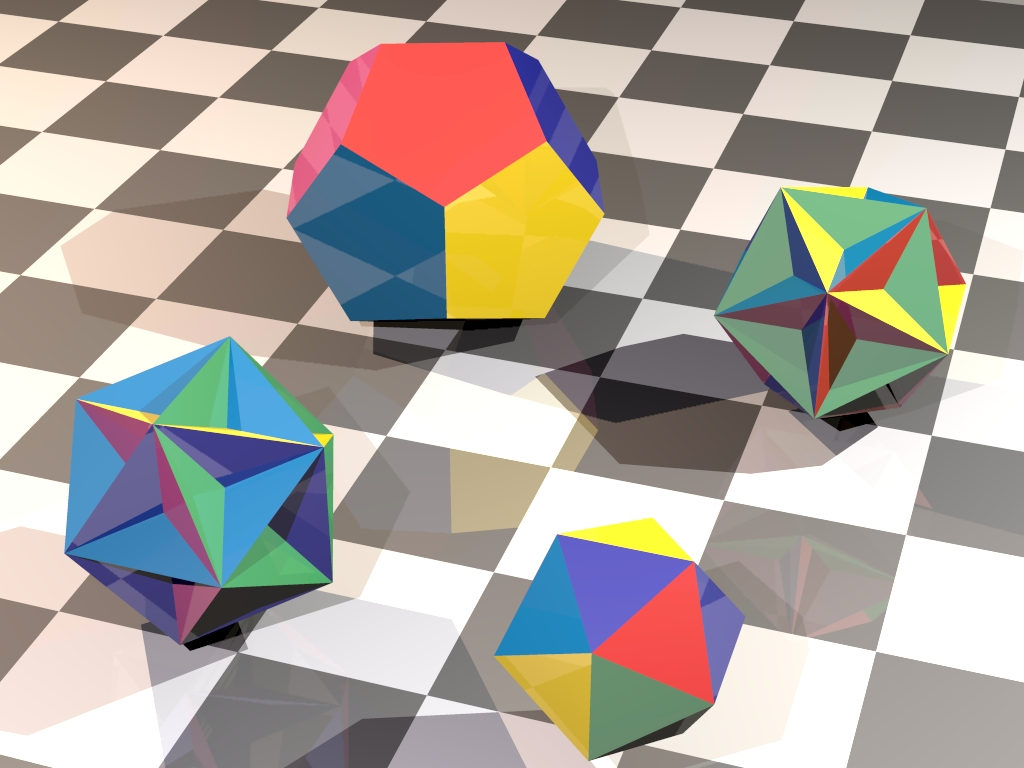
\includegraphics[width=.3\linewidth]{Images/Old_ART_Platonics.jpg} 
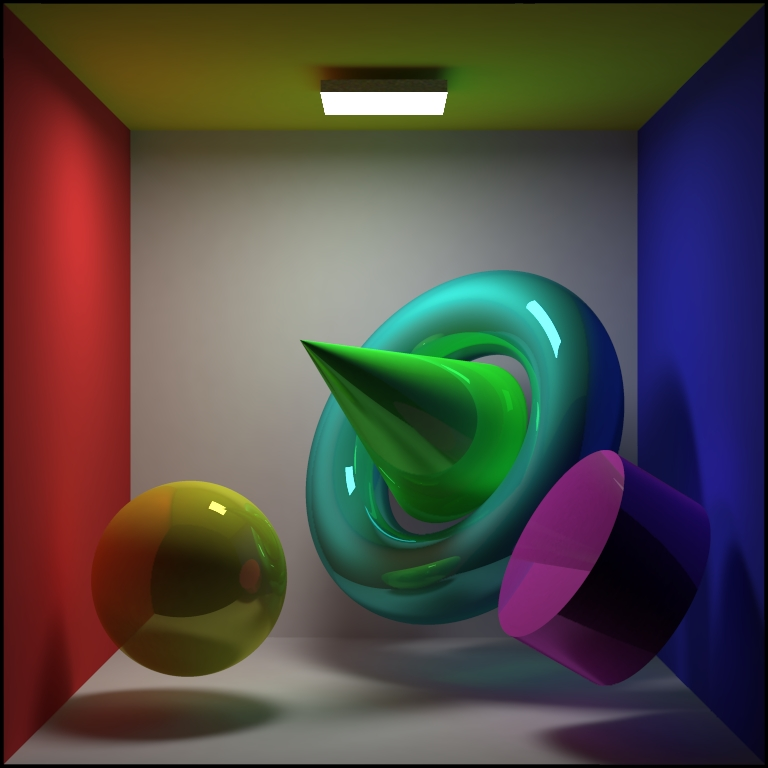
\includegraphics[width=.225\linewidth]{Images/Old_ART_Quadrics.jpg} 
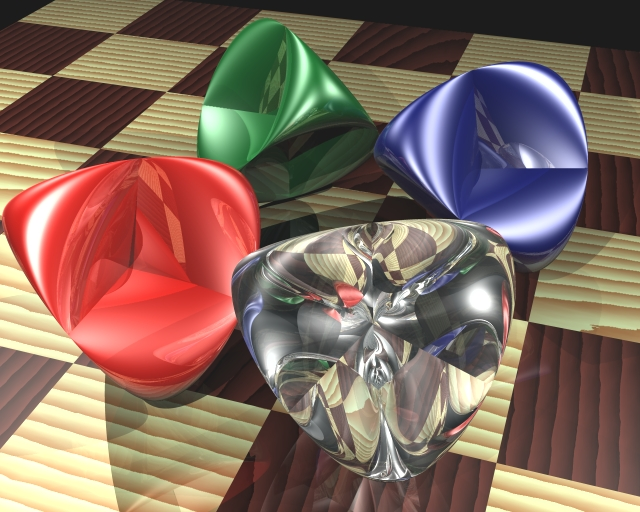
\includegraphics[width=.2825\linewidth]{Images/Old_ART_Steiners.jpg} 
\end{center}
\caption{
\label{fig:old_art} 
Images rendered with 0.x versions of ART in the approx.~timeframe 1996-2002. When handled correctly, even a fairly primitive renderer like a Whitted ray tracer could yield visually rich images. Note, however, that all reflections are perfect mirror reflections, or fake Phong highlights. The global illumination effects seen in the middle image were the result of a hybrid approach which pre-computed global illumination via stochastic radiosity: the final gather was still done via Whitted ray tracing. Also note how the rightmost image shows that even the 0.x series of ART already had a procedural shading language, which in this example was used to create the woodgrain texture on the chessboard.
}
\end{figure}

As a consequence of this background, the first versions of ART were heavily geared towards \command{rft}'s personal research topics. Visualisation of scene graphs was for a long time done via a comparatively primitive algorithm: classic Whitted ray tracing, \ie old school ray tracing which is only capable of dealing with perfectly diffuse surfaces and perfect mirrors, plus fake glossy highlights on Phong surfaces. Such a renderer does not compute global illumination, although GI could, at least in some sub-versions of early ART, be added via a stochastic radiosity pass. Point light sources were the norm; figure~\ref{fig:old_art} shows a few example images. 

\section{Middle Ages: ART 1.x}

Spectral rendering, including the ability to store spectral images in a special lossless HDR image file format called \filename{artraw} (see section~\ref{sect:propformats}), was added to the system starting around the year 1998. Polarisation support followed around the year 2000, and the initial version of \filename{artraw} was developed to store polarisation information: before that, Greg Ward's LogLuv HDR TIFF variant had been used as intermediate storage format between renderer and tonemapper. Bi-spectral capabilities were added in 2001. Due to the inclusion of polarisation and bi-spectral capabilities, the conceptual split between light and attenuation values discussed in section~\ref{sec:lightandattenuation} had to be introduced in the codebase around this time: this feature is conceptually one level above the actual spectral representation, and has been retained in more or less unchanged form since then.

By then, the system had become a collaborative effort between several persons at the institute, although \command{rft} was still the overall maintainer and designer. The version number was pushed to above 1 at some point after 2002, but ART was not publicly released then. This was mainly due to still being rather unfinished, and poorly documented: but there was always also a recurring theme of \emph{"we will do one more paper based on some advanced feature that no other renderer has, and then we will make it Open Source"}. Of course, by the time that particular paper had been done, there was always another one on the horizon, as convenient reason not to invest the considerable overhead needed to clean up the toolkit for release. After all, researchers are in the business of producing papers, not Open Source software.

When the ART version number was pushed to 1.x, \command{rft} had already left the institute, to work as senior researcher at the then newly opened VRVis graphics research centre. Although this centre is also located in Vienna, its research focus has always been more oriented towards interactive graphics, so an offline renderer like ART was not a research priority there. At VRVis, \command{rft} started work on an entirely new interactive rendering system called \emph{Aardvark}, which has  semantically very rich modelling capabilities: it has a number of features which are still ahead of its time even now, and which is still in production use there. As a result of \command{rft} having this new project on his hands, responsibility for ART changed over to the current maintainer, Alexander Wilkie, around 2003. Until 2008/2009, the 1.x series of ART continued to be used for work on publications by a sub-group at the Institute for Computer Graphics and Algorithms at Vienna Tech. 

In spite of spectral (and later even bi-spectral) rendering capabilities having been added, ART also continued to offer the functionality of rendering in colour space. This hybrid nature persisted through all ART 1.x versions: you could compile ART 1.x as an RGB renderer, but also as a spectral renderer which used $n$ fixed bins for its spectral representations, with 8, 16, 45 and 450\footnote{The mode with 450 spectral bins was intended for reference renderings with 1nm sampling distance across the visible range. It was never really used in practice, though, due to being extremely slow, and memory hungry. ART 2.x dropped this option.} bins being offered. Polarisation support was also a compile time option, and orthogonal to the chosen spectral resolution. This fact was cleverly hidden from the user: the actual renderer 'executable' \command{artist} was in fact a shell script, which picked the right executable (RGB, spectral, polarisation capable or not,...), based on user preferences. This was a hack, and made debugging quite difficult: but it did work reasonably well, and allowed one to compare the results obtained with different spectral sampling densities. Internally, a pseudo-polymorphic data type called \command{Colour} was used in all places that could refer to either a colour value or a spectrum: this macro placeholder was replaced with an appropriate structure at compile time\footnote{While this way of doing things is perfectly valid when working with ANSI C (at least purely from a technical viewpoint), the macro replacement of all instances of \command{Colour} was one of the reasons why ART 1.x executables were a pain to debug.}. The way this was done was via a simple \command{\#define}, such as \eg

\begin{verbatim}
#define Colour  Spectrum8
\end{verbatim}

to make all instances of \command{Colour} an 8 channel spectrum: \source{Spectrum8} was a simple ANSI C structure which contained 8 floats. This had the advantage that all instances of \command{Colour} could be statically allocated, as their size was known at compile time: no dynamic allocation and de-allocation of this internal representation of colours and spectra was needed. Due to the performance considerations discussed in section~\ref{sect:mixingCandC}, the representations of spectra and colours one could choose were implemented as low level C structures, and not ObjC classes, where polymorphism would have been available via the language.

\begin{figure}[htb]
\begin{center}
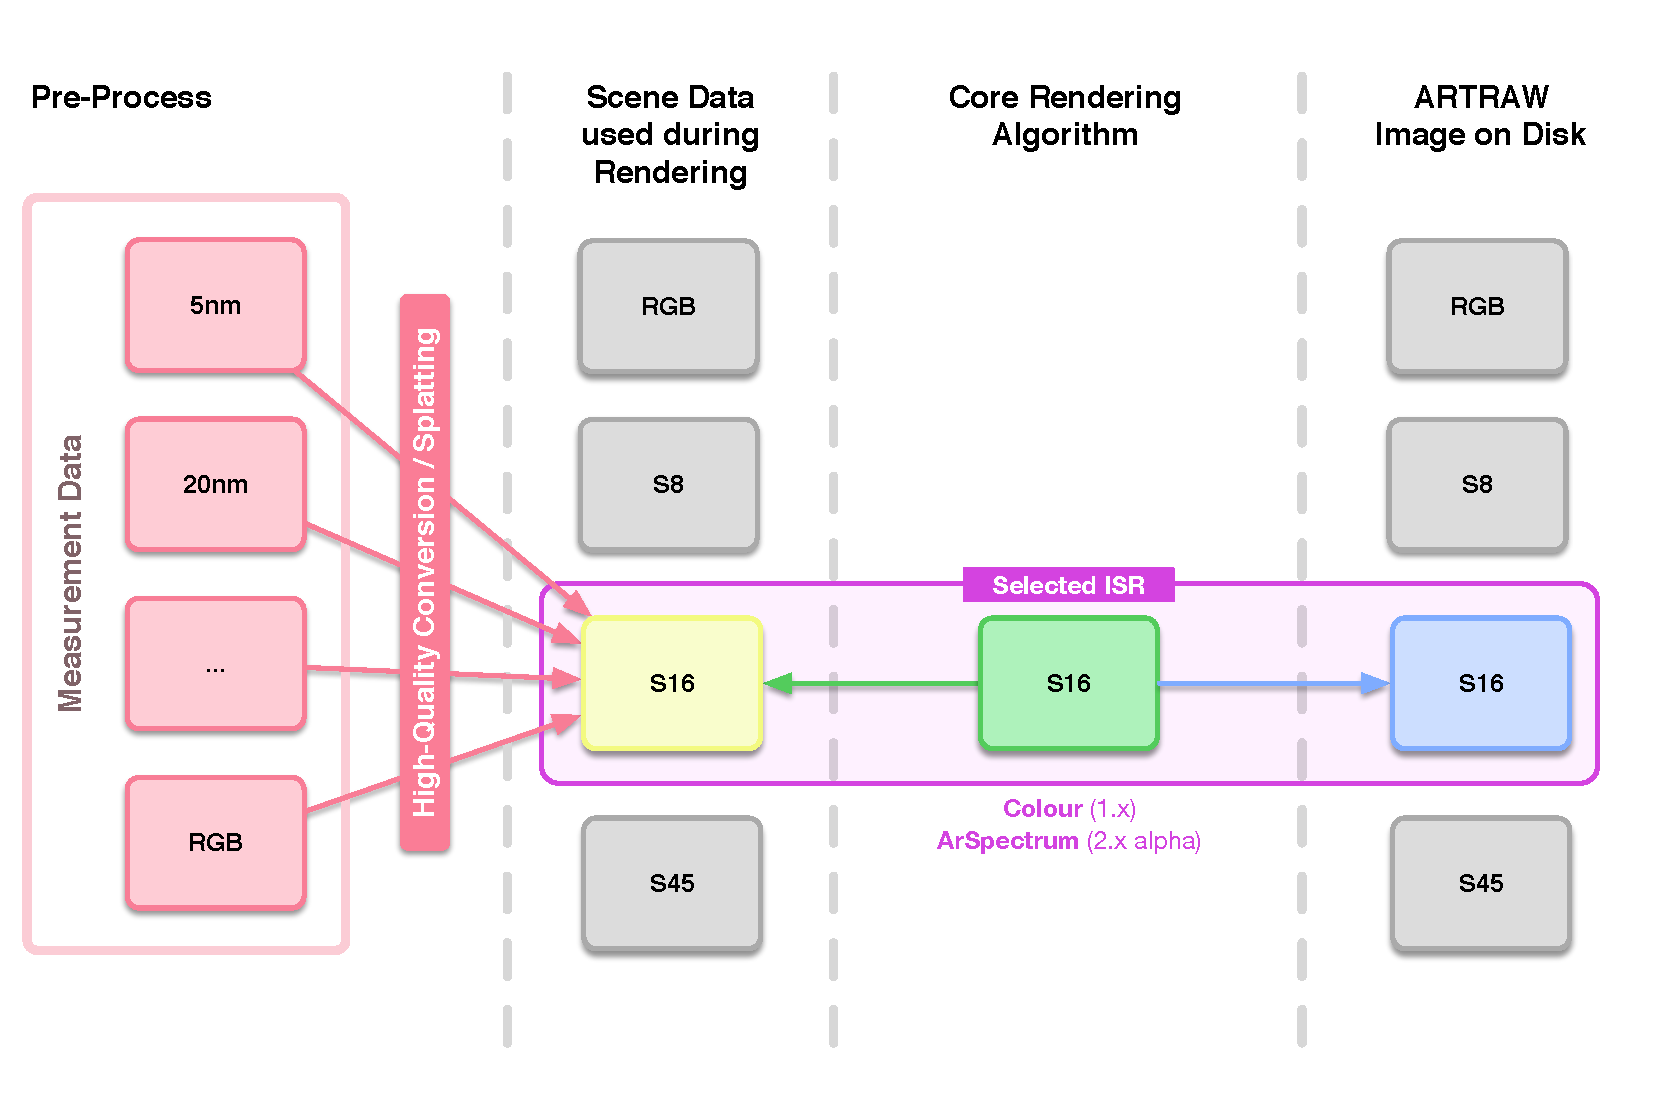
\includegraphics[width=.7\linewidth]{Images/Old_Spectral_Workflow.pdf} 
\end{center}
\caption{
\label{fig:old_spectralworkflow}
The logic of the fixed representation spectral workflow in ART 1.x, and early 2.x alpha. There is a wide range of input data that can be used in a scene description: but it all gets converted to a specific \emph{Internal Spectral Representation} (ISR), which is used during all computations, and which gets written into the result image. In this example, all input data is being reduced to the \command{Spectrum16} data type: as result, this data type exclusively gets used during rendering, and the resulting \filename{artraw} image also contains such data. The advantage of such an architecture is that no conversions, interpolation or splatting is being done during path tracing: all data is converted to the used ISR prior to rendering, and results are directly written to disk. Compare this to the current workflow, shown in figure~\ref{fig:spectralworkflow}.
}
\end{figure}

But "nailing down" the main spectral representation to one particular low-level C type (as opposed to a fancier solution with polymorphic ObjC types) was not only about performance: it was also implicitly about the data handling logic of the renderer itself. Polymorphism in the data structures which are used to describe colour or spectra in the core of the renderer is only useful if it serves a semantic purpose: but as figure~\ref{fig:old_spectralworkflow} shows, the logic of ART 1.x (and early 2.x) was to reduce all input data to a given internal representation on start up anyway, to avoid conversion calculations during the actual rendering loop. For this sort of logic, a simple C structure is perfectly sufficient, and actually desirable.

How was this \command{Colour} datatype used: the following code snippet is taken from Lambert surface material code of an ART 1.x version. First, the subnode which contains the actual colour (or spectral information) attached to the surface material is queried to return a \command{Colour} value for the given \command{hitInfo}, \ie a data structure which contains information on where the ray in question hit the object. The information in the \command{hitInfo} is \eg used to compute procedural texture results. Then, this \command{Colour} value is used to construct an \command{ArFilter} value, which is returned as the result of the method call: 

\begin{verbatim}
Colour  reflectionColour;
    
[ COLOUR_SUBNODE getColour: hitInfo : & reflectionColour ];

arfilter_c_init_nonpolarizing_f( & reflectionColour, outReflectionFilter );
\end{verbatim}

Note that \command{ArFilter} is the ART 1.x name for what is now known as \command{ArAttenuation} values (see section~\ref{sect:attenuation}). The idea behind the old name was that the information contained in it usually describes a \emph{filtering} of light\footnote{"Filtering" in the sense of light falling through a coloured filter, and being attenuated by it.}. This was later changed, as the term "filter" already has a set meaning in mainstream Computer Graphics, so ART 1.x usage of the term was needlessly confusing.

Overall, the \command{Colour}-based, "hardwired" hybrid colourspace and spectral ART 1.x worked reasonably well, with the only special cases in the codebase being caused by the distinction between polarising and non-polarising forms of the renderer. But unfortunately, after over ten years of not always perfectly guided development, the core software structure of ART 1.x, with its various idiosyncrasies, became more or less un-maintainable around 2007. Even worse was the fact that after a certain point, no single copy of the system which had all components in functional state existed. No version control for sources had been in use at the Vienna institute (in hindsight, this was a huge mistake), so merging was a manual process, and rarely done. Every research effort spawned a forked source tree, and a number of interesting research results were lost -- at least with regard to the source code used to generate the results found in the corresponding paper -- when such sub-versions of ART eventually were discarded along with old computers in the lab. In addition to all this, in spite of it working reasonably well when handled carefully, the hardwired spectral switching technique via \command{\#define} was clearly not an adequate long-term solution from a software engineering viewpoint: but as it was so ingrained in the system, nothing short of a major re-write would yield a useable alternative.


\section{Renaissance: early ART 2.x alphas}

In 2008, the maintainer of ART moved to Charles University in Prague. By then, several physically based open source rendering systems had been published, most notably the seminal \command{pbrt}. However, none of the available systems were (bi-)spectral, or had polarisation capabilities. Nor did any system use a stable and documented spectral image file format. As these topics continued to be of considerable research interest to the maintainer, and as such capabilities are very hard to retro-fit into other more mainstream rendering systems (such as \command{pbrt}), the decision was made to keep ART around, and to start a complete overhaul of the system. However, this overhaul went along a gradual path: with regard to spectral rendering, early alpha versions of ART 2.x were essentially a more sane and stable re-implementation of the dual colourspace/spectral capabilities seen in the ART 1.x series, and which are illustrated in figure~\ref{fig:old_spectralworkflow}. It was only the later 2.x alphas which dropped the capability to render in colourspace, and which switched to the current pure spectral rendering model that is discussed in section~\ref{sect:currentart}.

\subsection{Internal Spectral Representations}
\label{sect:CCTs}
It was not before the complete re-write that was to become ART 2.x that the \emph{internal spectral representation} (ISR for short) of colour values and/or spectra became something you could actually switch in a running instance of ART. In the early alphas of 2.x, a polymorphic data type that can resolve to either form during runtime was introduced: the structure which is now called \command{ArSpectrum}. Admittedly, \command{ArSpectrum} is not a perfect name for this data type (just like the name for its exact counterpart \command{Colour} in ART 1.x was not) -- after all, the content of this data structure can also be a colour value, and not just a spectrum. But the English language seems to lack an expression which succinctly describes both types of data at the same time.

Technically, \command{ArSpectrum} is a struct that contains a single \source{void *} pointer which references the actual data. The actual data can, in turn, be one of the ISRs supported by ART. Because of this, instances of \command{ArSpectrum} can only be dynamically created and deleted via their associated \command{spc\_alloc()} and \command{spc\_free()} functions. Static instances of \source{ArSpectrum} do not make sense, and do not work. All functions that operate on \command{ArSpectrum} instances are re-directions to the appropriate functions for the "native" content of the \command{ArSpectrum} struct. Figure~\ref{fig:arcolour} shows an overview of this.

\begin{figure}[htbp]
\begin{center}
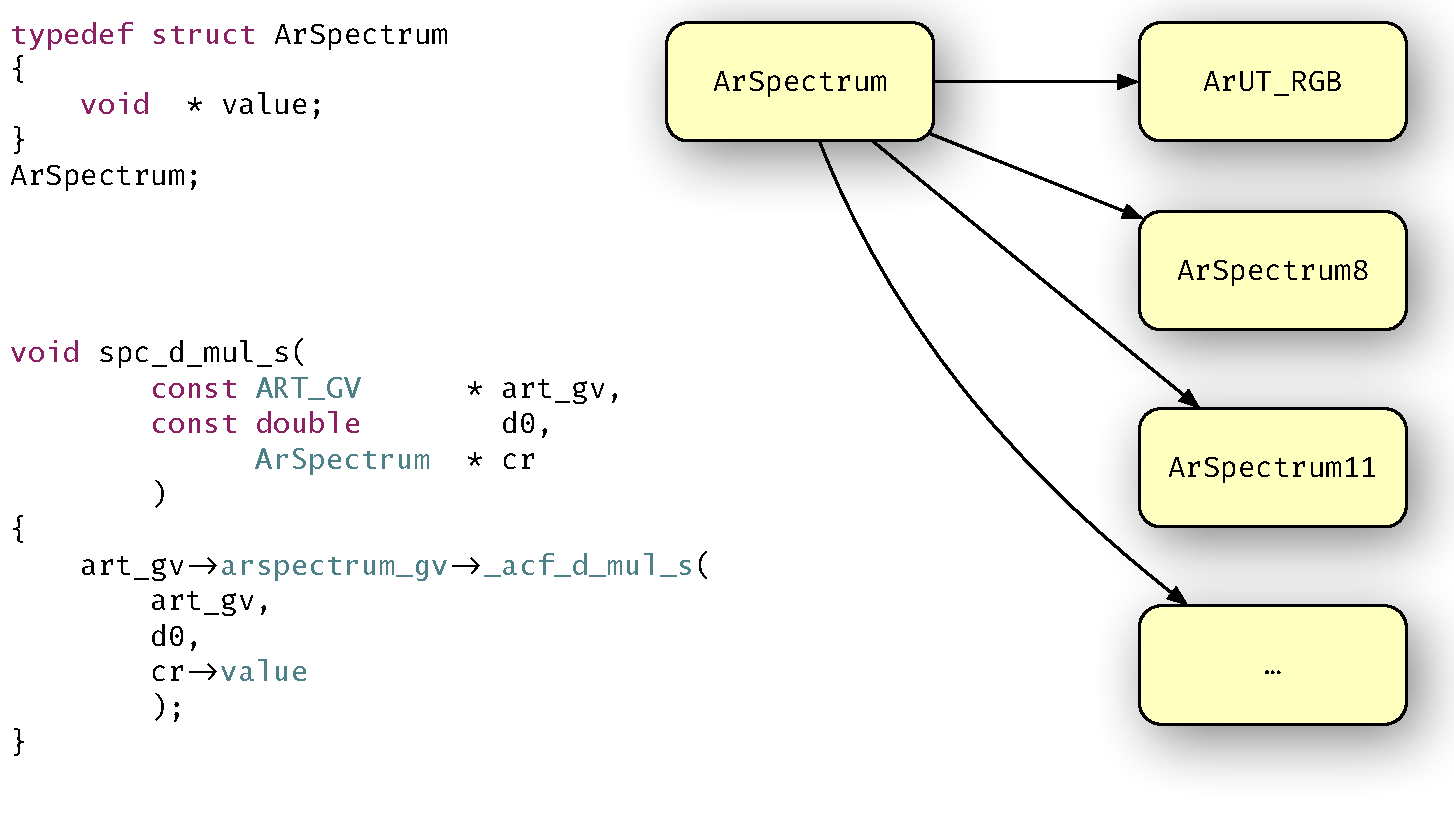
\includegraphics[width=.5\linewidth]{Images/ArSpectrum.pdf} 
\end{center}
\caption{
\label{fig:arcolour} 
Graphical illustration of the \source{ArSpectrum} wrapper data type. The \source{void} pointer inside the struct can point to any of a number of ISR types (listed on the right). Functions that operate on \source{ArSpectrum} arguments use a function pointer that is stored in the \source{ART\_GV} protected global state, and changed accordingly when the ISR is being switched, to call the correct function to operate on the \source{void *} contents of the struct. In effect, this approach is a form of object oriented programming and encapsulation, only done via pure C and function pointers for performance and portability reasons.
}
\end{figure}

The following ISRs are currently available in ART: see figure~\ref{fig:art_isr_ranges} for an illustration of their respective ranges. If you want to compare their performance, render the Macbeth colour charts found in the gallery section.

\begin{enumerate}
\item \textbf{\source{ArSpectrum8}}, command line flag \textbf{-s8v}: an 8 band visible range spectrum with 40nm spacing. Intended as reasonable option in terms of \source{artraw} file size, but which still delivers quite passable colour accuracy. This setting is the default.
\item \textbf{\source{ArSpectrum11}}, command line flag \textbf{-s11e}: an 11 band spectrum with 40nm spacing, which covers both the near UV as well as the visible range. The bands in this spectral type correspond to the bands used in the Hosek sky dome model, and were originally defined for this purpose. Suitable for extended range data which does not have any sharp spectral features.
\item \textbf{\source{ArSpectrum18}}, command line flag \textbf{-s18v}: an 18 band visible range spectrum with 20nm spacing. A higher accuracy option for visible range images.
\item \textbf{\source{ArSpectrum46}}, command line flag \textbf{-s46e}: a 46 band spectrum with 10nm spacing, which covers both the near UV as well as the visible range. A high-accuracy counterpart to \textbf{s11}, which can also be used for reference images in the visible range.
\end{enumerate}

This particular selection of ISRs is only weakly hard-coded into ART -- adding more would be a fairly small effort. 

\begin{figure}[htb]
\begin{center}
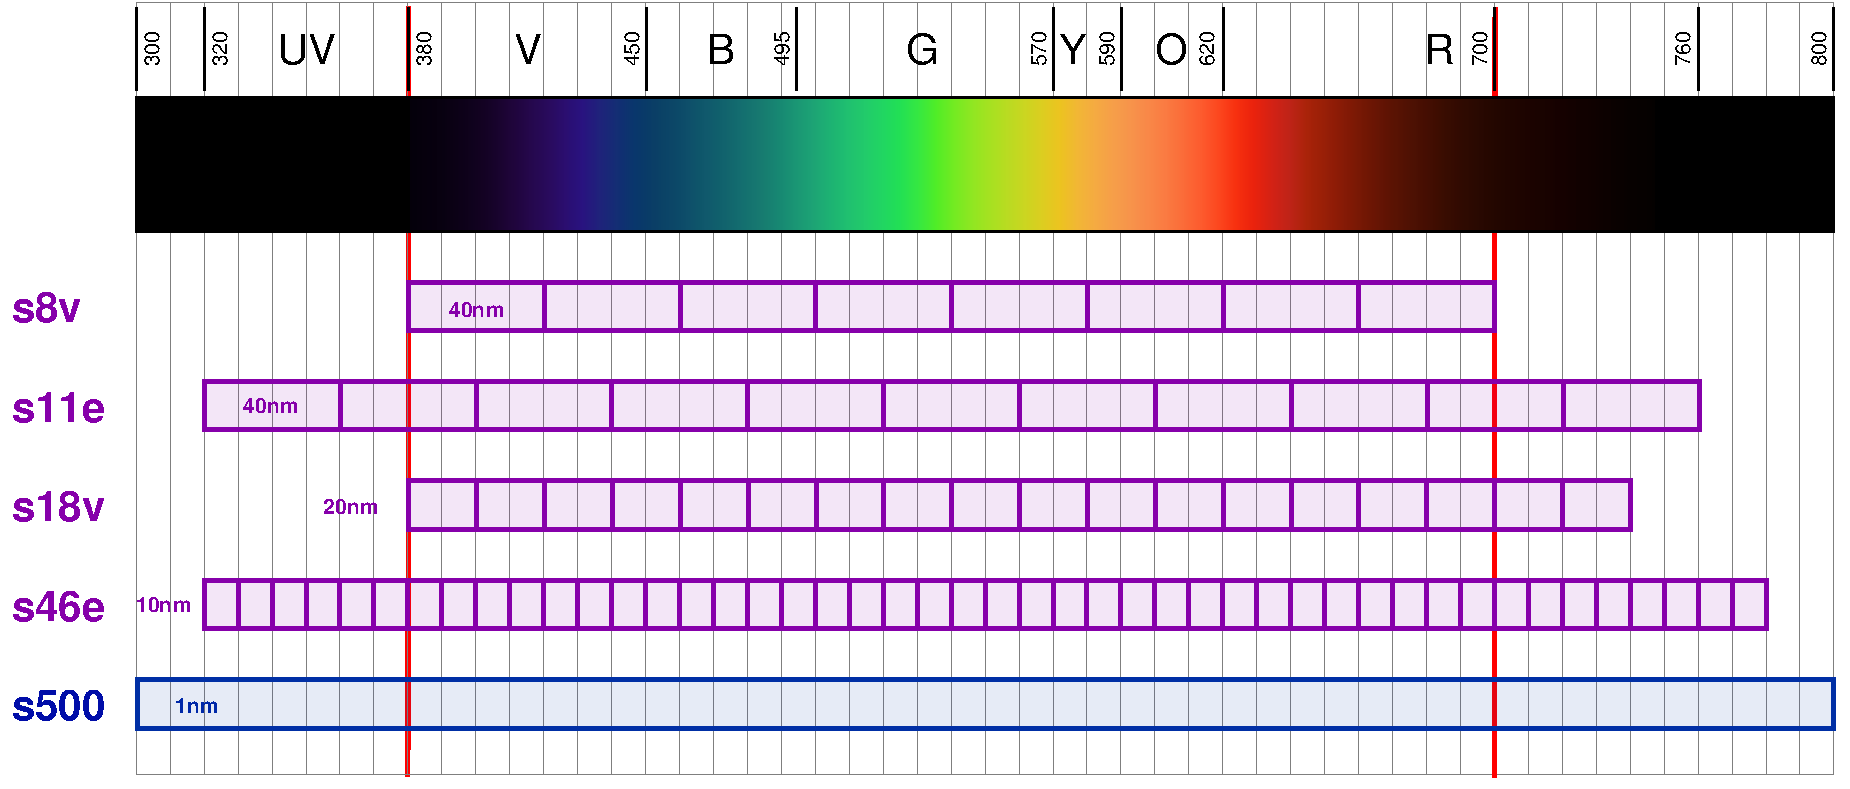
\includegraphics[width=.8\linewidth]{Images/ART_ISR_Ranges.pdf} 
\end{center}
\caption{
\label{fig:art_isr_ranges} 
Spectral ranges of the current ART ISRs, plus the internal \textbf{s500} type: the red vertical lines denote what can be seen as the "main visible range". The CIE XYZ standard observer functions are defined to beyond 800nm, but only have tiny values beyond 700nm. For instance, the cut-off of \textbf{s8v} at 700nm is motivated by the fact that for equal energy illumination, and the 1932 CIE XYZ primaries, the energy above 700nm accounts for the following percentages in an XYZ triplet: $(0.15\%,0.06\%,0.00\%)$. \textbf{s18v} adds two bands that go to 740nm, which accounts for $(0.14\%,0.05\%,0.00\%)$ of the remaining energy, \ie practically the entire missing energy. \textbf{s500} is intended as an internal catch-all datatype, and as such has to go beyond all actual spectral ranges found in \source{artraw} images.
}
\end{figure}

Once they started up, the early ART 2.x alphas used one of these ISR types for all its internal calculations that involved basic "colour or spectral values", exactly as ART 1.x had used the \command{Colour} data type. All user-specified data were converted to the accuracy of the currently active ISR prior to rendering, and images generated while running in a particular mode were saved in their native ISR form, so that no data is destroyed after rendering (see section~\ref{sect:propformats} on \filename{artraw}, which is the file format that is capable of storing whatever ISR data is put into it). Figure~\ref{fig:old_spectralworkflow} gives a schematic of this process. Switching the ISR involves changing all the function pointers which are used to manipulate the contents of \command{ArSpectrum} instances. Also, certain in-built constants (such as the values for black and white, or zero and unit radiance/reflectance, respectively) have to be re-created to match the current ISR. The place where one can find the source for all this is the \command{ColourAndSpectra} library in the Foundation part of ART.

Because of the low-level nature of this switching process, it is not feasible to switch the ISR once a scene has been loaded, or during rendering. If the user specifies that a file be rendered in a particular ISR that differs from the current standard of \command{ArSpectrum8}, the first thing the \command{artist} command-line renderer does is to switch ISR, before doing anything else. The command line options for the \command{artist} renderer which switch to a particular ISR are \option{-rgb}, \option{-s8}, \option{-s11}, \option{-s16} and \option{-s45}, respectively.

The approach to directly use the ISRs during path tracing calculations, and to reduce all data to the ISR on loading, was ultimately dropped for two reasons:

\begin{enumerate}
\item As the development of physically based rendering progressed, it made less and less sense to retain the colourspace rendering capabilities which ART 1.x had had.
\item It became clear that fixed width spectral representations do have their uses, but not in the core of a renderer. There, either monochrome or Hero sampled spectra are much more appropriate.
\end{enumerate}

As we will see in the next section, ART 2.x actually retains the capability of being switched to a particular ISR. However, internally, mono or Hero sampling is used for all spectral data, and the choice of ISR now only affects the spectral sampling rate of the output image. The early ART 2.x alphas were, in spite of their transient nature, still used for work on a number of publications during the 2010-2016 timeframe. 

\section{Modernity: Spectral Path Tracing in Current ART 2.x}
\label{sect:currentart}

Low level handling of spectral quantities in ART path tracing is internally done via the \emph{Hero wavelength sampling} approach which was first demonstrated in the Manuka renderer of Weta Digital: as of 2018, this appears to be the current state of the art in spectral rendering. The path tracer of ART 2.x is no longer able to internally work in colour space, which from the viewpoint of physical correctness is hardly a negative thing: all path tracing is now exclusively done with spectral data. An overview of the new workflow can be seen in figure~\ref{fig:spectralworkflow}.

\begin{figure}[htb]
\begin{center}
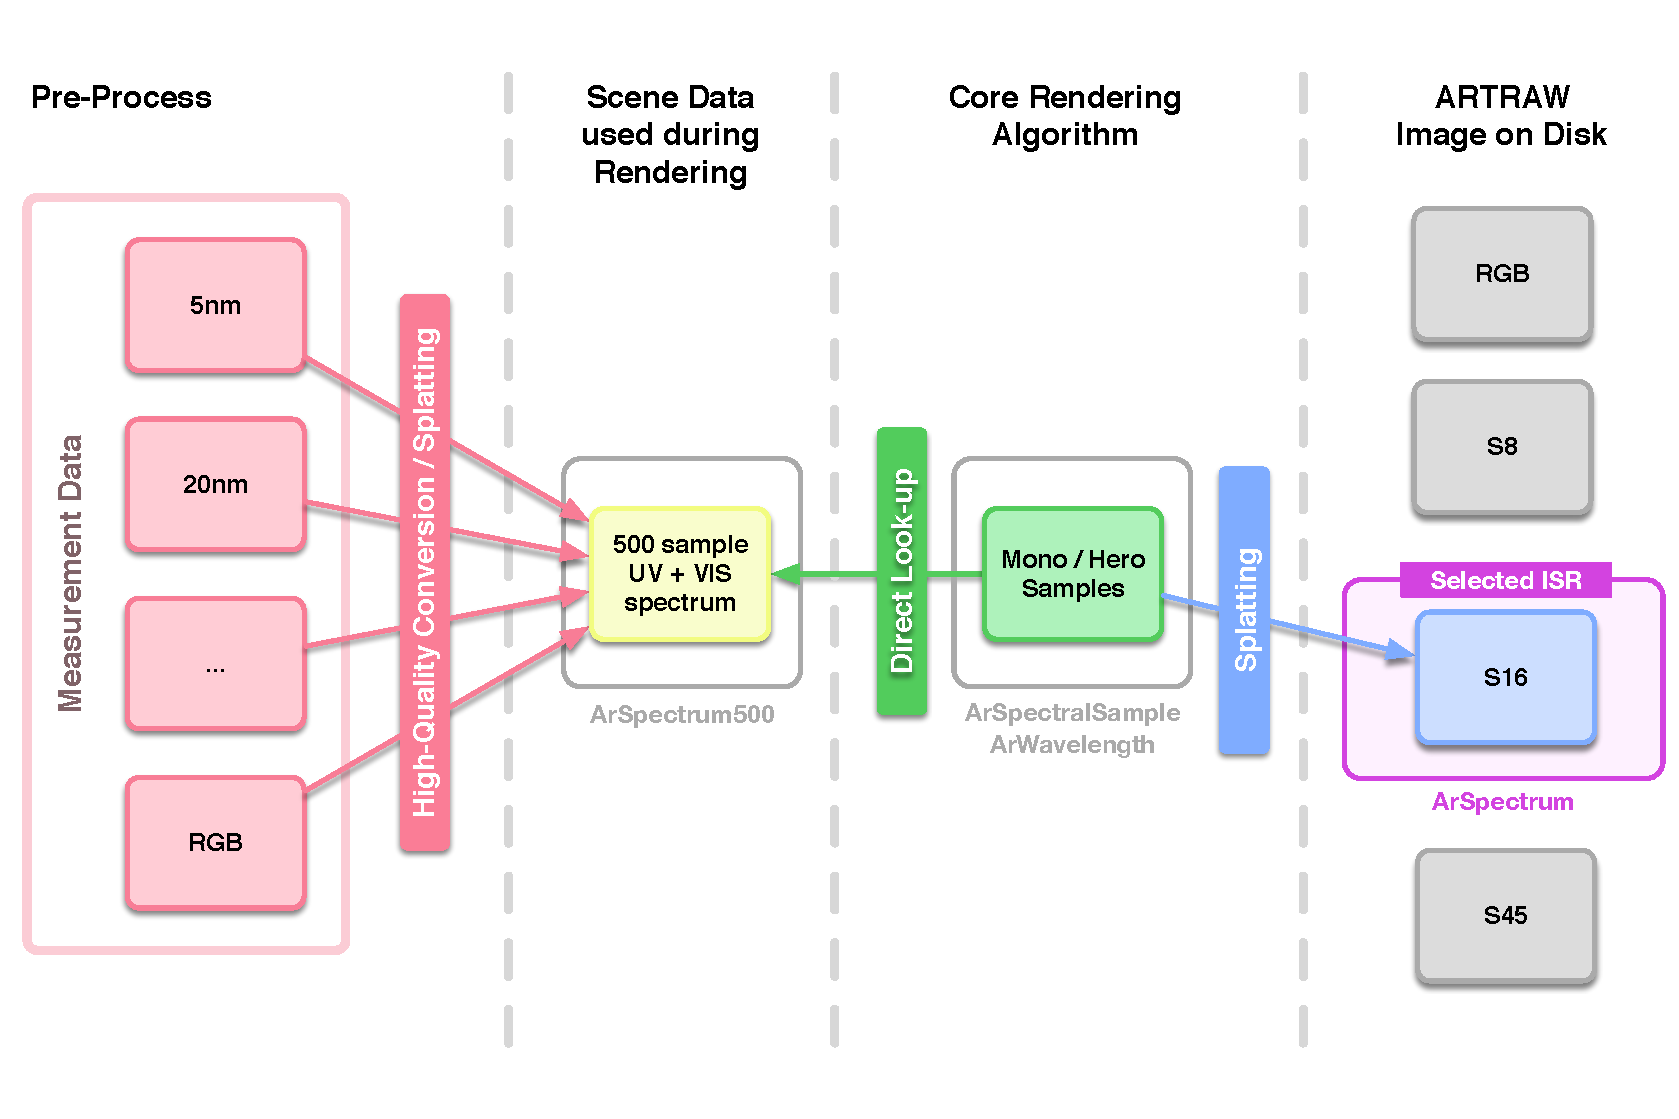
\includegraphics[width=.7\linewidth]{Images/Spectral_Workflow.pdf} 
\end{center}
\caption{
\label{fig:spectralworkflow}
The current spectral workflow in the ART path 2.x tracer. Note that the user still selects an ISR (underlaid in purple), like in the ART 1.x workflow shown in figure~\ref{fig:old_spectralworkflow}: however, this now only affects the spectral resolution of the output image. For path tracing, all other spectral data is actually \emph{upsampled} to an internal form with 1nm spectral resolution. The advantage of this is that random wavelength sampling can directly grab any wavelength bin, and use it without any interpolation or further processing. The downside of this technique is memory usage, which is typically not an issue unless the scene contains image maps. Results of the core rendering loop are splatted into the result \filename{artraw}. Note that this result file can also contain colour space data, if the user selects this. Also note that the inclusion of polarisation information is orthogonal to the \source{ArSpectrum} type: the actual data stored in an \filename{artraw} are \source{ArLight} values, which can be either plain or polarising. See figure~\ref{fig:csla_subsystem} for an overview. 
}
\end{figure}


Internally, the data type \command{ArSpectralSample}, with its accompanying type \command{ArWavelength} to describe the sampling wavelength(s), is now being used for all spectral samples taken by the path tracer. Once an estimate has been obtained, these samples are splatted into the result \filename{artraw}. Hero sampling is conceptually simpler in a number of ways than the previously used fixed-width spectral representations: and it is also faster, more suited for polarisation rendering, and less biased than the old techniques. Hero sampling is being used by default: but for debugging and verification purposes, ART can actually be switched to "monochrome mode", where only a single wavelength is traced. The workflow shown in figure~\ref{fig:spectralworkflow} remains the same if this is done.

On a higher level, ART 2.x continues to use the concept of light and attenuation values discussed in section~\ref{sec:lightandattenuation}, and which was first introduced in ART 1.x. For use within the path tracer, the corresponding sample types \source{ArLightSample} and \source{ArAttenuationSample} were introduced.
 
Once the switch to Hero rendering was complete, the entire switching machinery behind the polymorphic \command{ArSpectrum} data type from the early 2.x alphas could theoretically have been removed from ART, as it is not needed for direct rendering purposes anymore. However, the notion of selecting a "master ISR" which all spectral data can default to was actually retained: mainly because the sub-system was already there, well tested, and stable. It was reduced in importance, though, as can be seen from figure~\ref{fig:spectralworkflow}: it now only affects the resolution of the output image. In principle, the infrastructure of being able to switch the entire \command{ArSpectrum} infrastructure between specific ISR types is now considerable overkill for just selecting a data type used for \command{artraw} content: as such, this sub-system would not have been written "from scratch" the way it is for the purpose it is being used for now. But as long as it does not get in the way of new functionality (and it is hard to see how it would do that), it stays in the toolkit.

\chapter{Light and Attenuation}
\label{sec:lightandattenuation}

As stated before, due to having to deal with polarisation and bi-spectral data, ART internally has to make a distinction between light values (\source{ArLight} structs) and light attenuation values (\source{ArAttenuation}
structs). There are also corresponding types for single or Hero wavelength samples taken from either. In this section, we explain some of the internal workings of these data types, and the relationship between them. We briefly discuss naming, start with a general overview of \source{ArAttenuation}, and then discuss the issues specific to the polarisation support within ART.

\begin{figure}[htb]
\begin{center}
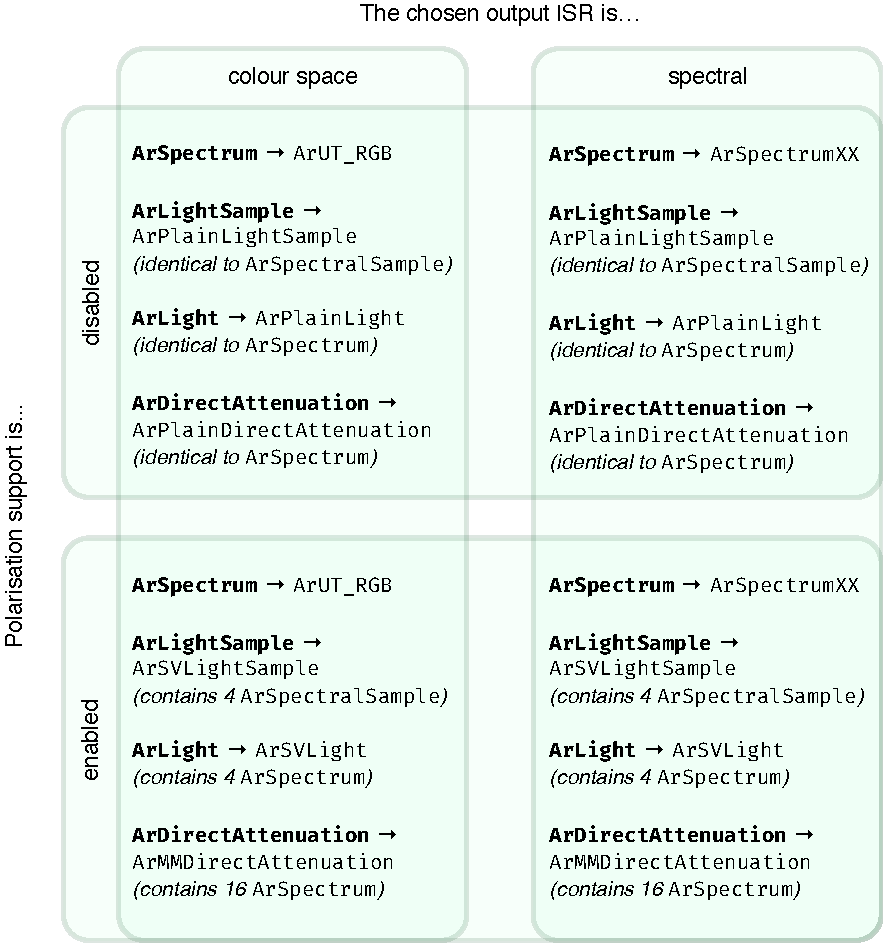
\includegraphics[width=.7\linewidth]{Images/CSLA_Subsystem.pdf} 
\end{center}
\caption{
\label{fig:csla_subsystem} 
Overview of the respective contents of all the switchable data types of the CSLA subsystem (\source{ArSpectrum}, \source{ArLightSample}, \source{ArLight} and \source{ArDirectAttenuation}) for the various operation modes of ART. \source{ArSpectrumXX} stands for any of the concrete spectral ISRs, such as \eg\source{ArSpectrum45}.
}
\end{figure}

\section{The \source{ArAttenuation} Data Type}

One of the physical effects ART is designed to handle is fluorescence: this means that apart from directly attenuating the incident energy, any light-matter interaction can also potentially transfer energy from one waveband to another. So for the old ART 1.x renderer, and the early 2.x alphas, which both worked on entire spectra at once, a counterpart to \source{ArLight} which was capable of encoding this energy-shifting behaviour was needed. The path tracer in ART 2.x does not actually use \source{ArAttenuation} anymore, and instead works with wavelength-sampling \source{ArAttenuationSamples}, and explicit wavelength shifts to handle fluorescence: for such surfaces, it also integrates over the wavelength shifting dimension. So technically speaking, the \source{ArAttenuation} data type described here is no longer needed: but as the code was functional, it made no sense to explicitly delete it.

\subsection{Naming Conventions: Attenuation \vs Reflectance}
\label{sect:attenuation}
In ART, we use the term \emph{attenuation} (of light) as a general term for the changes in intensity that light undergoes upon interaction with matter. In most rendering systems, expressions like \emph{reflectance} are used for this sort of quantity. However, in ART, the attenuation data type is intended to encode \emph{all} interactions of light with matter, and this goes beyond mere reflectance: scattering events (\eg Rayleigh scattering in the atmosphere) are one example of this. The \source{ArAttenuation} data type also encodes fluorescence effects, which involve energy transfer between different wavelengths -- yet another concept that goes beyond normal reflectance.

\subsection{\source{ArAttenuation} Contents}

In order to handle fluorescence, an \source{ArAttenuation} struct contains two main components:

\begin{enumerate}
\item an \source{ArCrosstalk} structure, which describes the frequency/colour band crosstalk found in fluorescent materials, and
\item an \source{ArDirectAttenuation} structure, which is the classical reflectance value. 
\end{enumerate}

Figure~\ref{fig:arattenuation} gives a graphical overview of this. Notable points are that the direct attenuation (but only that -- the fluorescence described by the crosstalk is a non-polarising phenomenon) can be switched between a polarisation-aware form and a plain one, and that flags are used to make certain operations more efficient.

\begin{figure}[htb]
\begin{center}
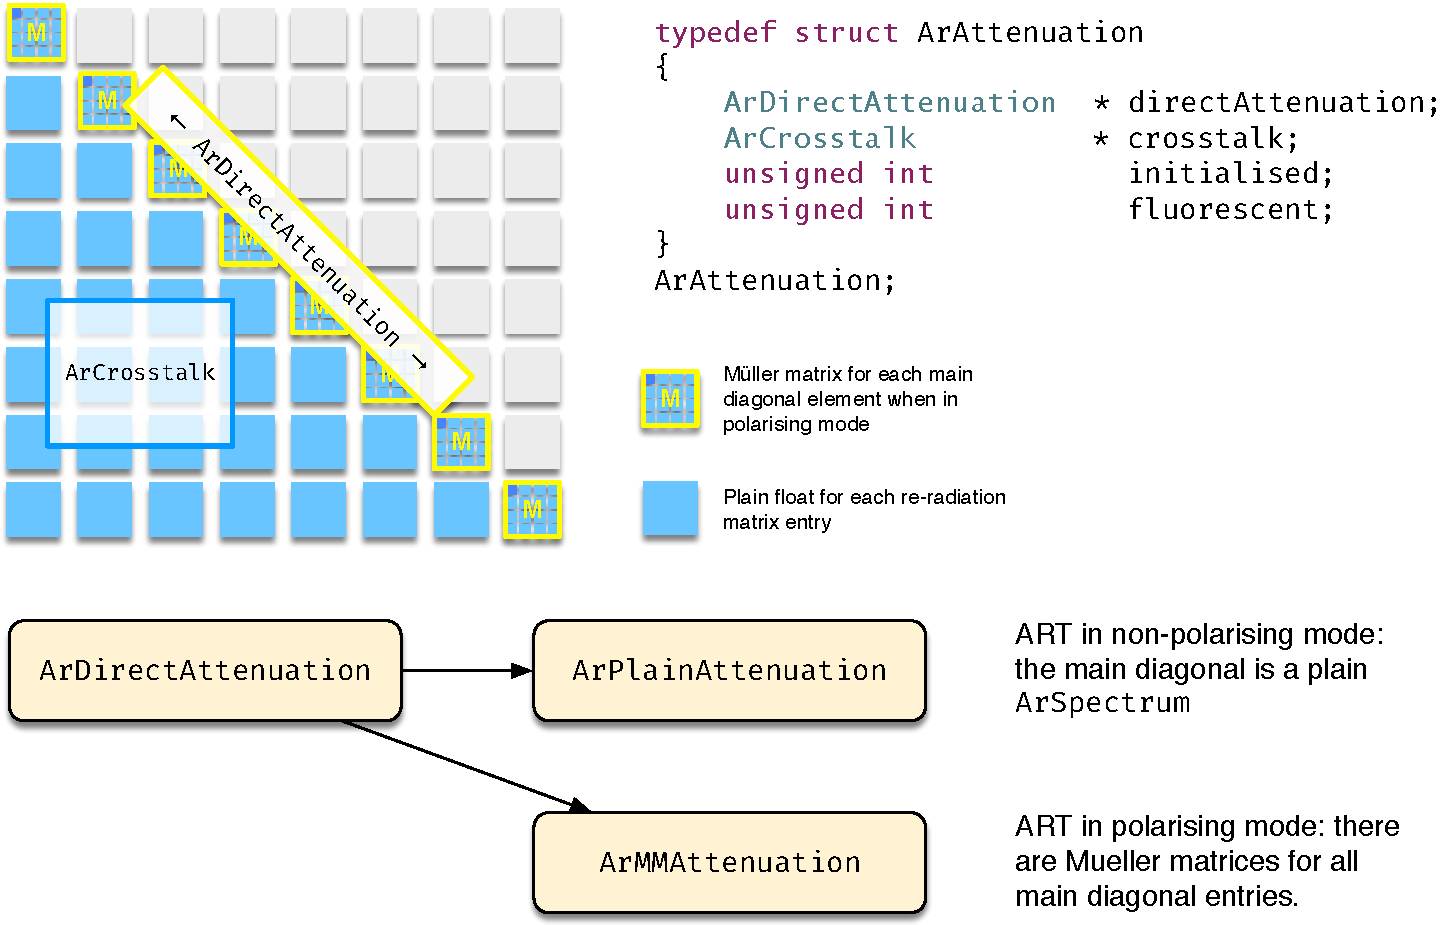
\includegraphics[width=.6\linewidth]{Images/ArAttenuation.pdf} 
\end{center}
\caption{
\label{fig:arattenuation} 
\source{ArAttenuation} contains two components, the crosstalk data structure, and the direct attenuation. The \source{ArDirectAttenuation} struct switches between plain and a polarisation-aware mode and, like \source{ArLight}, expands to a single \source{ArSpectrum} value for the non-polarising mode. The fluorescence crosstalk is always just an array of float values, since it is a purely non-polarising phenomenon.
}
\end{figure}

\section{\source{ArLight}}
Compared to \source{ArAttenuation}, \source{ArLight} is a rather simple data type. For a plain rendering system without
polarisation support it just contains a single \source{ArSpectrum} instance: nothing more than a colour value or a spectrum is needed to describe a radiance value. If the system is switched to polarisation-aware mode, it contains a C structure with 4~elements of type \type{ArSpectrum} to encode the 4~components of the Stokes Vector, as well as a single reference frame.

\begin{figure}[htb]
\begin{center}
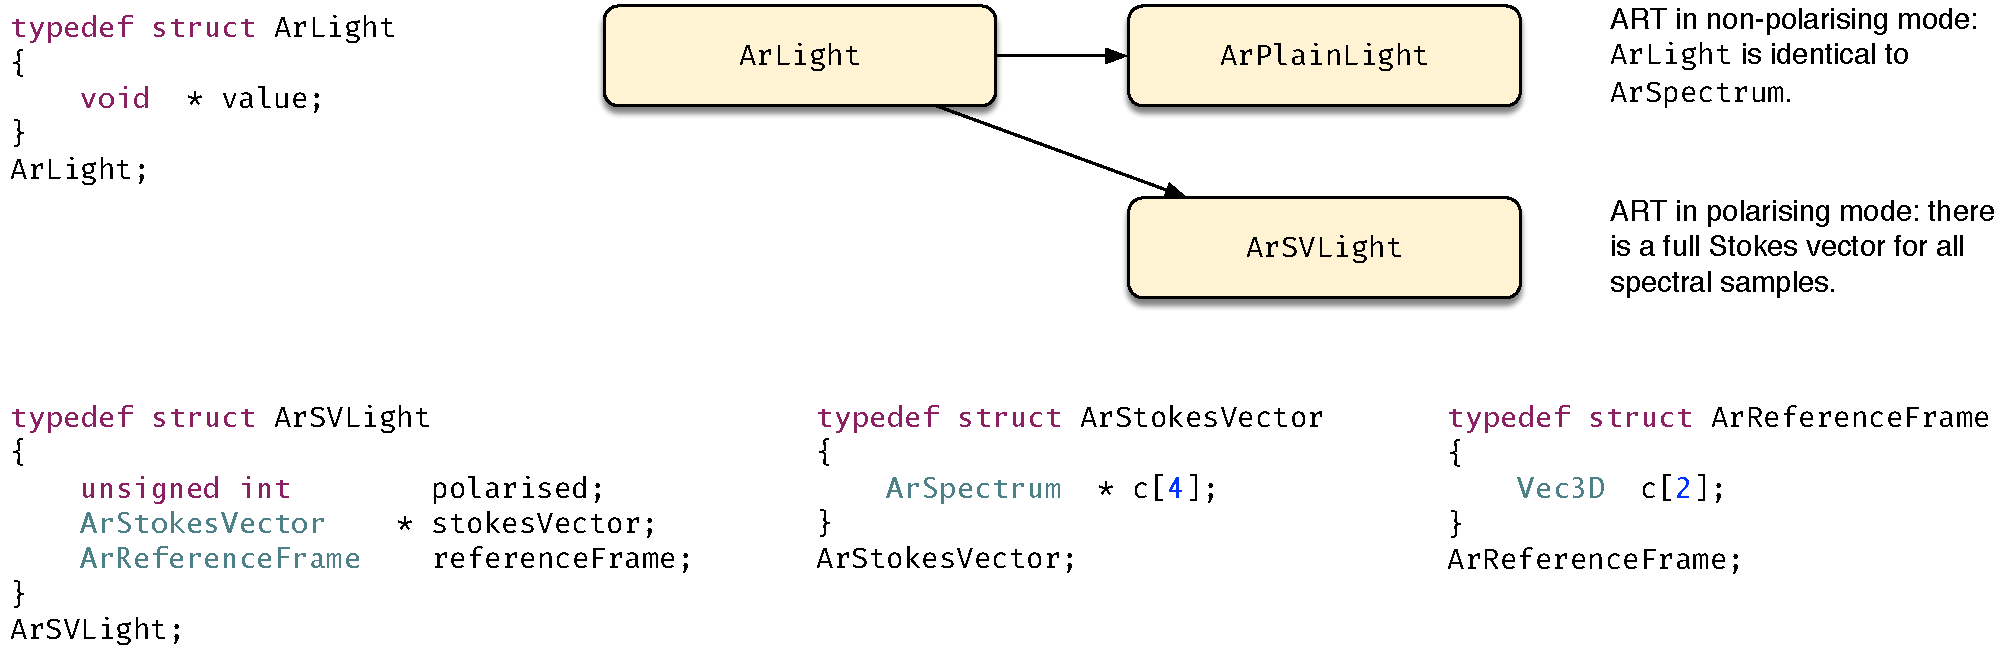
\includegraphics[width=.9\linewidth]{Images/ArLight.pdf} 
\end{center}
\caption{
\label{fig:arlight} 
\source{ArLight} contains a \source{void} pointer to allow a switch between plain and polarisable data structures. The plain light data structure is an \source{ArSpectrum} value, while the polarisation-aware version, \source{ArSVLight}, contains a Stokes Vector representation and a reference frame.
}
\end{figure}

Like \source{ArAttenuation}, \source{ArLight} values are no longer directly used during the path space computations of ART. But unlike the attenuation struct, it still has a very important purpose: \source{artraw} result images have pixels which are \source{ArLight} structs. Each \source{ArLightSample} which is computed by a path is splatted into the result \source{ArLight} for the pixel it belongs to.

\section{Polarisation Support}

Polarisation-aware routines for the manipulation of light and reflectance data are significantly more computationally costly than their plain counterparts. In practice, this means that it is infeasible to permanently activate this sort of functionality in a general purpose rendering engine such as ART. So in order to support rendering with polarised light, both light and attenuation data have to be switchable between plain and polarisation-aware versions. By default, \source{artist} runs in plain mode, and for those executables where such a functionality makes sense, the polarisation mode can be activated via the \source{-p} command line flag.

\begin{figure}[htbp]
\begin{center}
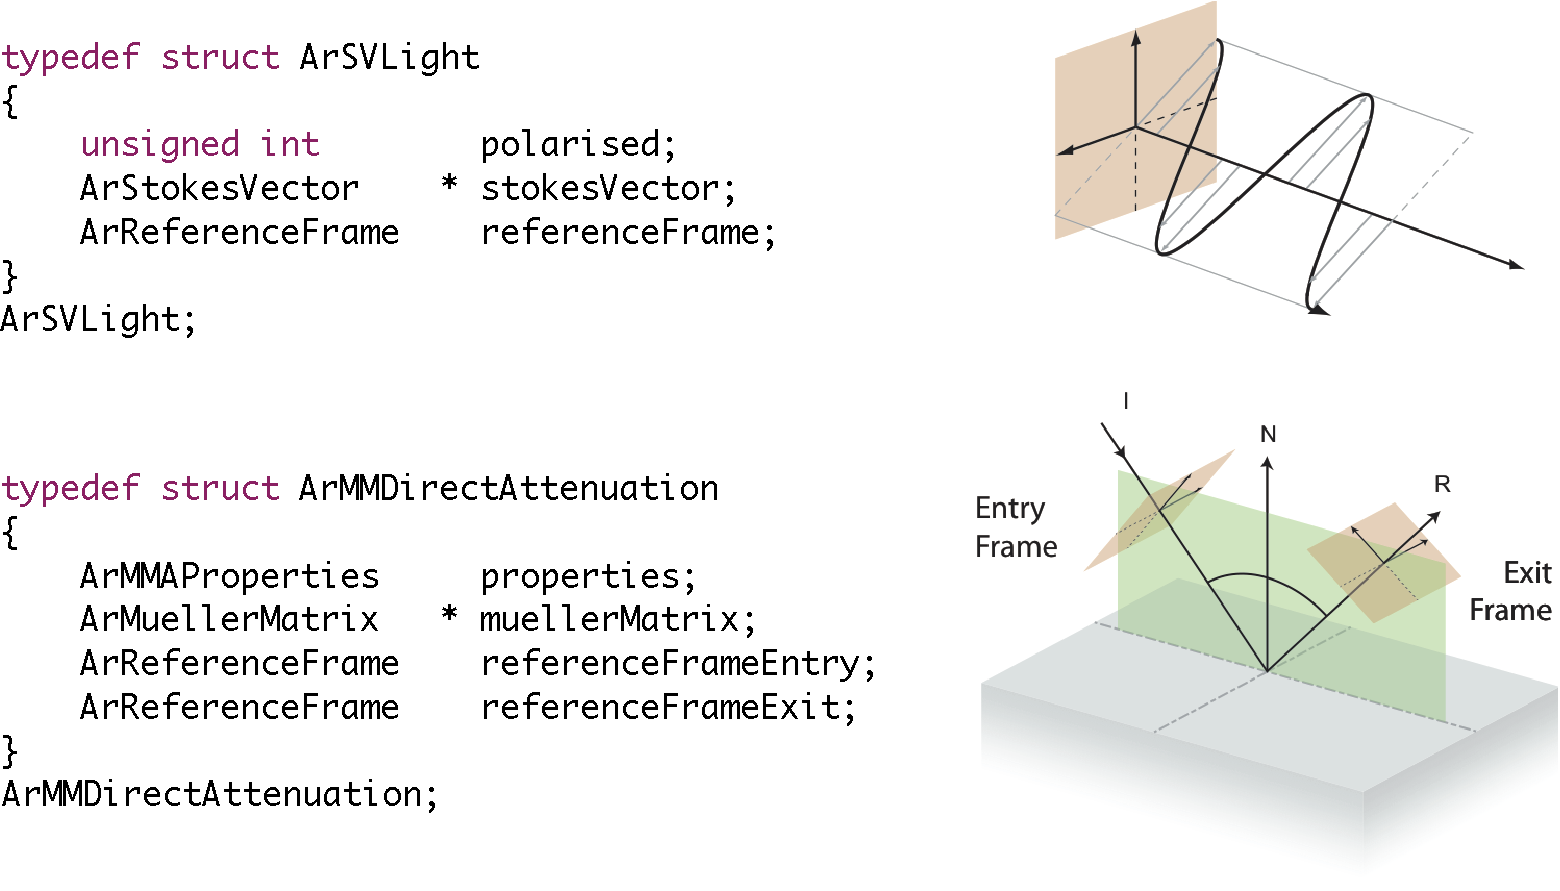
\includegraphics[width=.7\linewidth]{Images/C_Structures.pdf} 
\end{center}
\caption{
\label{fig:c_structs} 
The two polarisation-aware data structures \source{ArSVLight} and \source{ArMMDirectAttenuation} shown side by side. Note that the Stokes Vector structure has a single reference frame, while the one for the Mueller Matrix has two.
}
\end{figure}

To make this switching possible, the remaining other CSLA types like \source{ArLight} \ea are, exactly like \source{ArSpectrum}, also shell structures with a single \source{void} pointer inside: their inner workings, and their initialisation, are practically identical those of \source{ArSpectrum} discussed in section~\ref{sect:CCTs}. The similarities include the fact that the switch to the desired mode has to be made very early during the start-up sequence of ART, and that the mode cannot be easily changed once the system is running. A difference is that the switch they perform is not done between several ISRs, but between plain versions of the data structure in question (\source{ArPlainLight} and \source{ArPlainDirectAttenuation}, which are both just \source{ArSpectrum} in disguise), and their polarisation-aware counterparts (\source{ArSVLight} and \source{ArMMDirectAttenuation}, where SV stands for "Stokes Vector", and MM for "Mueller Matrix"). Figure~\ref{fig:csla_subsystem} shows a diagram which explains the contents of each of the top-level structures for the various operation modes of ART.

\section{Using CSLA Values in ART Rendering Code}

Contrary to what the somewhat involved preceding paragraphs might suggest, usage
of such data types within ART is very straightforward, since a considerable effort is made to
conceal all the inner workings of the switching CSLA system. Function names follow an assembly-like operator naming scheme, and function signatures are kept as similar as possible between the various CSLA types. Examples of light and attenuation functions would be:
\begin{verbatim}
arlight_dl_mul_l( art_gv, d0, l0, lr );
\end{verbatim}
for a function which scales a light value \source{l0} by a scalar \source{d0} and stores the result in a separate light struct \source{lr}, or
\begin{verbatim}
arattenuation_a_mul_a( art_gv, a0, ar );
\end{verbatim}
which multiplies (\ie concatenates) two attenuations \source{a0} and \source{ar}, and stores the result in the second one. The internal workings of these two functions are considerably different for plain and polarisation-aware rendering modes. But in any client code, such as surface reflectance code, one only ever has to use the functions as they stand, and the internals of the CSLA subsystem pick the right functions on the fly during code execution.

The only real price one has to pay for this polymorphic behaviour is that static allocations of \source{ArSpectrum}, \source{ArLight} and \source{ArAttenuation} instances are not possible (and arguably, this is not a high price to pay). All instances have to be dynamically created and destroyed via the appropriate functions, like such:

\begin{verbatim}
ArLight  * l0 = arlight_alloc( art_gv );

arlight_d_init_l( art_gv, 0.5, l0 );

<l0 gets used>

arlight_free( art_gv, l0 );
\end{verbatim}

Note the presence and usage of the ubiquitous \source{art\_gv} structure as first argument for all these functions. That structure, which is of the type \source{struct ART\_GV}, encapsulates the state of a running ART instance in a totally opaque fashion, \ie such that no code in any of the modules can directly manipulate state variables that are not defined within the same module. In this way, global variables (such as the function pointers needed for the CSLA functionality) can exist in a perfectly safe and re-entrant fashion: they can not be altered, except via well-defined manipulator functions.

\chapter{Specification of CSLA Values in ARM Files}


Also, a distinction has to
be made between the so-called \emph{ISR computation types} -- which are
the representations used \emph{internally} by the toolkit for ISR
values, or their components -- and the data types which are \emph{externally} available in
order to specify colour and spectral values. For colours these two categories overlap to some degree (RGB values are available both as ISR and as a modelling construct), for spectra they do not.

In ART scene description files, colour values, light and reflectances can be
specified in two different ways: in a conventional colour space such as
\option{RGB} or \option{CIE XYZ}, or as spectral quantities. While the first
option is usually far more convenient for modelling purposes, the latter allow physically accurate rendering with measured surface reflectances. Data specified in different systems can, to the extent that this is sensible from a technical viewpoint\footnote{See the caveat about using RGB colours in a spectral renderer at the end of this section for details.}, be freely mixed within a scene. The representations available in ARM files are described in
table~\ref{tab:representations}.

\begin{table}[htb]
\centering
\begin{tabular}{|>{\ttfamily}p{0.4\linewidth}|p{0.55\linewidth}|}
\hline
CONST\_COLOUR\_RGB(r,g,b)
CONST\_COLOUR\_RGB\_CS(r,g,b,cs)
&
RGB tristimulus values, without and with a colour space reference. If no colour space is specified, the colour is  assumed to be in the default colour space used during rendering (\ie a floating reference).
\\ \hline

CONST\_COLOUR\_CIEXYZ(X,Y,Z)       
CONST\_COLOUR\_CIExyY(x,y,Y)
& CIE XYZ and x,y,Y values 
\\ \hline

\parbox[t]{0.9\linewidth}{CONST\_COLOUR\_RSSPECTRUM( \\
start wavelength, \\
sample distance, \\
maximum value, \\
sample0, \\
sample1, \\
\ldots, \\
RSS\_END )} 
& 
Regularly spaced spectral values. This type of data is what measurement devices usually produce. Wavelengths have to be tagged with the appropriate physical units, \eg~380~\variable{NANOMETERS}, or 380.0~\variable{NM} for short.

Note that the \emph{maximum value} argument is not the maximum value of the given
samples (which could be easily computed), but the theoretical maximum value of
the whole spectrum. This information is needed to normalise the spectrum. After
the sample values (which are of type \type{double}), there MUST follow the
end tag \variable{RSS\_END} as last argument of the macro, otherwise the vararg
routines will be unable to process the sample list. A symptom of such an
omission can be a \command{make: error 139} (\ie runaway vararg)
message during an \filename{arm->art} translation.
\\ \hline

\parbox[t]{0.9\linewidth}{CONST\_COLOUR\_PSSPECTRUM( \\
maximum value, \\
sample0, \\
sample1, \\
\ldots, \\
PSS\_END ) }
&
Point sampled spectra. These can have arbitrarily spaced samples and are basically a polyline, which is more convenient for manually constructed spectra.

The samples are of type \variable{PNT\_2D}, and the maximum value argument has the same
significance as for regularly spaced spectra. As above, specifying the end tag
\variable{PSS\_END} is crucial. \\ \hline
\end{tabular}
\caption{ARM file constructor macros for the basic CLA data types available in ART. The \source{CONST\_} prefix signifies that these are, as the name implies, constant values which take immutable float values as input -- as opposed to the corresponding variable CLA data types of the ART shading language, which take expressions that evaluate to floats as input.}
\label{tab:representations}
\end{table}

The main drawback of spectral colour specifications is that one usually needs a
library of real material measurements to work with, since the manual construction of
spectra for a specific purpose is usually very difficult and non-intuitive (and usually also nonsensical from a physics viewpoint anyway). But such material measurements are hard to come by, since the devices needed to obtain them (\ie Spectro-Photometers) are not that common. Because of this, we provide a library which includes the spectral reflectance values of the glossy Munsell Book of Colour\textsuperscript{\scriptsize \textregistered}, the RAL Classic\textsuperscript{\scriptsize \textregistered} colour collection and transmission measurements of the Roscolux\textsuperscript{\scriptsize \textregistered} filters for entertainment lighting with ART. Between them, these spectra should provide ample data for users wishing to model scenes with realistic reflectances and transmission values. Access to these spectra is made comparatively easy by the fact that their names are canonical forms of the respective colour atlas coordinates, as can be seen in the following ARM scene examples:

\begin{verbatim}
green_diffuse_surface =  LAMBERT_REFLECTOR( MUNSELL_025G_08_04 );
ral_classic_surface =    LAMBERT_REFLECTOR( RAL_8008 );
\end{verbatim}

As far as using RGB values in ARM files is concerned, it should be noted that it is intrinsically problematic to provide colour values as input to a spectral renderer, since the construction of a corresponding spectrum is an ambiguous and badly conditioned problem. Also, this reconstruction functionality (which existed in a somewhat more extensive ART 1) is currently only partially active in ART 2: the current solution only really makes sense for emissive RGB values, as it is based on adding up the RGB spectra of LCD monitor primaries. So the resulting spectra are not really plausible when used as reflectance values.


%%%%%%%%%%%%%%%%%%%%%%%%%%%%%%%%%%%%%%%%%%%%%%%%%%%%%%%%%%%%%%%%%%%%%%%%%%%%%%%%%%%%%%%%%%%








%%% Local Variables: 
%%% mode: latex
%%% TeX-master: "ARTforNewbies"
%%% End: 



\clearemptydoublepage
\bibliography{ARTforNewbies}
%\clearemptydoublepage
%\listoftables
\end{document}
